\PassOptionsToPackage{unicode=true}{hyperref} % options for packages loaded elsewhere
\PassOptionsToPackage{hyphens}{url}
%
\documentclass[]{article}
\usepackage{lmodern}
\usepackage{amssymb,amsmath}
\usepackage{ifxetex,ifluatex}
\usepackage{fixltx2e} % provides \textsubscript
\ifnum 0\ifxetex 1\fi\ifluatex 1\fi=0 % if pdftex
  \usepackage[T1]{fontenc}
  \usepackage[utf8]{inputenc}
  \usepackage{textcomp} % provides euro and other symbols
\else % if luatex or xelatex
  \usepackage{unicode-math}
  \defaultfontfeatures{Ligatures=TeX,Scale=MatchLowercase}
\fi
% use upquote if available, for straight quotes in verbatim environments
\IfFileExists{upquote.sty}{\usepackage{upquote}}{}
% use microtype if available
\IfFileExists{microtype.sty}{%
\usepackage[]{microtype}
\UseMicrotypeSet[protrusion]{basicmath} % disable protrusion for tt fonts
}{}
\IfFileExists{parskip.sty}{%
\usepackage{parskip}
}{% else
\setlength{\parindent}{0pt}
\setlength{\parskip}{6pt plus 2pt minus 1pt}
}
\usepackage{hyperref}
\hypersetup{
            pdftitle={Desregulación molecular inducida por tratamiento con alcohol en células precursoras neurales a partir de células embrionarias humanas pluripotentes},
            pdfauthor={Marina Ballesteros},
            pdfborder={0 0 0},
            breaklinks=true}
\urlstyle{same}  % don't use monospace font for urls
\usepackage[margin=1in]{geometry}
\usepackage{color}
\usepackage{fancyvrb}
\newcommand{\VerbBar}{|}
\newcommand{\VERB}{\Verb[commandchars=\\\{\}]}
\DefineVerbatimEnvironment{Highlighting}{Verbatim}{commandchars=\\\{\}}
% Add ',fontsize=\small' for more characters per line
\usepackage{framed}
\definecolor{shadecolor}{RGB}{248,248,248}
\newenvironment{Shaded}{\begin{snugshade}}{\end{snugshade}}
\newcommand{\AlertTok}[1]{\textcolor[rgb]{0.94,0.16,0.16}{#1}}
\newcommand{\AnnotationTok}[1]{\textcolor[rgb]{0.56,0.35,0.01}{\textbf{\textit{#1}}}}
\newcommand{\AttributeTok}[1]{\textcolor[rgb]{0.77,0.63,0.00}{#1}}
\newcommand{\BaseNTok}[1]{\textcolor[rgb]{0.00,0.00,0.81}{#1}}
\newcommand{\BuiltInTok}[1]{#1}
\newcommand{\CharTok}[1]{\textcolor[rgb]{0.31,0.60,0.02}{#1}}
\newcommand{\CommentTok}[1]{\textcolor[rgb]{0.56,0.35,0.01}{\textit{#1}}}
\newcommand{\CommentVarTok}[1]{\textcolor[rgb]{0.56,0.35,0.01}{\textbf{\textit{#1}}}}
\newcommand{\ConstantTok}[1]{\textcolor[rgb]{0.00,0.00,0.00}{#1}}
\newcommand{\ControlFlowTok}[1]{\textcolor[rgb]{0.13,0.29,0.53}{\textbf{#1}}}
\newcommand{\DataTypeTok}[1]{\textcolor[rgb]{0.13,0.29,0.53}{#1}}
\newcommand{\DecValTok}[1]{\textcolor[rgb]{0.00,0.00,0.81}{#1}}
\newcommand{\DocumentationTok}[1]{\textcolor[rgb]{0.56,0.35,0.01}{\textbf{\textit{#1}}}}
\newcommand{\ErrorTok}[1]{\textcolor[rgb]{0.64,0.00,0.00}{\textbf{#1}}}
\newcommand{\ExtensionTok}[1]{#1}
\newcommand{\FloatTok}[1]{\textcolor[rgb]{0.00,0.00,0.81}{#1}}
\newcommand{\FunctionTok}[1]{\textcolor[rgb]{0.00,0.00,0.00}{#1}}
\newcommand{\ImportTok}[1]{#1}
\newcommand{\InformationTok}[1]{\textcolor[rgb]{0.56,0.35,0.01}{\textbf{\textit{#1}}}}
\newcommand{\KeywordTok}[1]{\textcolor[rgb]{0.13,0.29,0.53}{\textbf{#1}}}
\newcommand{\NormalTok}[1]{#1}
\newcommand{\OperatorTok}[1]{\textcolor[rgb]{0.81,0.36,0.00}{\textbf{#1}}}
\newcommand{\OtherTok}[1]{\textcolor[rgb]{0.56,0.35,0.01}{#1}}
\newcommand{\PreprocessorTok}[1]{\textcolor[rgb]{0.56,0.35,0.01}{\textit{#1}}}
\newcommand{\RegionMarkerTok}[1]{#1}
\newcommand{\SpecialCharTok}[1]{\textcolor[rgb]{0.00,0.00,0.00}{#1}}
\newcommand{\SpecialStringTok}[1]{\textcolor[rgb]{0.31,0.60,0.02}{#1}}
\newcommand{\StringTok}[1]{\textcolor[rgb]{0.31,0.60,0.02}{#1}}
\newcommand{\VariableTok}[1]{\textcolor[rgb]{0.00,0.00,0.00}{#1}}
\newcommand{\VerbatimStringTok}[1]{\textcolor[rgb]{0.31,0.60,0.02}{#1}}
\newcommand{\WarningTok}[1]{\textcolor[rgb]{0.56,0.35,0.01}{\textbf{\textit{#1}}}}
\usepackage{longtable,booktabs}
% Fix footnotes in tables (requires footnote package)
\IfFileExists{footnote.sty}{\usepackage{footnote}\makesavenoteenv{longtable}}{}
\usepackage{graphicx,grffile}
\makeatletter
\def\maxwidth{\ifdim\Gin@nat@width>\linewidth\linewidth\else\Gin@nat@width\fi}
\def\maxheight{\ifdim\Gin@nat@height>\textheight\textheight\else\Gin@nat@height\fi}
\makeatother
% Scale images if necessary, so that they will not overflow the page
% margins by default, and it is still possible to overwrite the defaults
% using explicit options in \includegraphics[width, height, ...]{}
\setkeys{Gin}{width=\maxwidth,height=\maxheight,keepaspectratio}
\setlength{\emergencystretch}{3em}  % prevent overfull lines
\providecommand{\tightlist}{%
  \setlength{\itemsep}{0pt}\setlength{\parskip}{0pt}}
\setcounter{secnumdepth}{0}
% Redefines (sub)paragraphs to behave more like sections
\ifx\paragraph\undefined\else
\let\oldparagraph\paragraph
\renewcommand{\paragraph}[1]{\oldparagraph{#1}\mbox{}}
\fi
\ifx\subparagraph\undefined\else
\let\oldsubparagraph\subparagraph
\renewcommand{\subparagraph}[1]{\oldsubparagraph{#1}\mbox{}}
\fi

% set default figure placement to htbp
\makeatletter
\def\fps@figure{htbp}
\makeatother


\title{Desregulación molecular inducida por tratamiento con alcohol en células
precursoras neurales a partir de células embrionarias humanas
pluripotentes}
\author{Marina Ballesteros}
\date{4/9/2020}

\begin{document}
\maketitle

{
\setcounter{tocdepth}{2}
\tableofcontents
}
\begin{enumerate}
\def\labelenumi{\arabic{enumi}.}
\tightlist
\item
  Datos del estudio
\end{enumerate}

Los datos del análisis se han cargado desde la base de datos Gene
Expression Omnibus (GEO). El conjunto de datos seleccionado se
identifica con el número de adhesión: \textbf{GSE56906}.

El estudio que generó dichos datos investiga el efecto del alcohol
(EtOH) en el desarrollo de células madre neurales derivadas desde
células madre de embriones humanos. Existen indicios de que el alcohol
interviene negativamente en el desarrollo de las células madre neurales.
Para corroborar estos indicios, se han cultivado células madre
embrionarias durante cinco días en un medio de inducción neural (NIM). A
continuación, los agregados neuronales fueron sembrados en placas
recubiertas con poli-L-ornitina/laminina y cultivados con NIM durante
siete días adiccionales para desarrollar la estructura de roseta
neuronal. Después de siete días, las rosetas neurales fueron desalojadas
y luego replateadas para la expansión de las células precursoras
neurales (NPC) durante 3-5 días.

Los microarrays utilizados para este experimento fueron del siguiente
tipo: Affymetrix Human Genome U133 Plus 2.0 Array.

\#\#Preparación del ambiente de trabajo

Antes de empezar con el análisis y a manejar la enorme cantidad de datos
y ficheros que ello conlleva, crearé tres carpetas para la organización
del mismo:

\begin{itemize}
\tightlist
\item
  La carpeta principal del análisis será ``Effect of alcool in ESC
  differentiation'', la cual también será mi directorio de trabajo.
\item
  Una carpeta llamada \textbf{data} para almecenar todo tipo de datos
  del experimento y en los cuales basaré mi análisis. En esta carpeta
  guardaré los archivos \emph{.CEL} y el archivo \emph{targets}, en el
  cual se decribirán los factores de estudio y sus niveles.
\item
  En la carpeta \textbf{results} guardaré todos los resultados obtenidos
  en el análisis.
\item
  La carpeta \textbf{figures} servirá para almacenar todo tipo de
  imágenes y figuras generadas durante el análisis.
\end{itemize}

\hypertarget{lectura-de-los-datos}{%
\subsection{Lectura de los datos}\label{lectura-de-los-datos}}

En el experimento se han analizado 10 muestras, las cuales se analizan
en torno a dos factores: el tipo celular y el tipo de tratamiento
durante la diferenciación celular. Los niveles de dichos factores son
los siguientes:

Para el factor \textbf{tipo celular} existen tres niveles:

\begin{itemize}
\tightlist
\item
  Células madre embrionarias (ESC) indiferenciadas \emph{H1 p40}
\item
  Células neurales en forma de roseta \emph{H1 Rosett}
\item
  Células progenitoras neurales (NPC) \emph{NPC H1}
\end{itemize}

Para el factor \textbf{tipo de tratamiento} existen dos niveles:

\begin{itemize}
\tightlist
\item
  Células diferenciadas sin tratamiento con alcohol \emph{EtOH 0}
\item
  Células diferenciadas bajo tratamiento con alcohol \emph{EtOH 20}
\end{itemize}

Una tabla que recoge todas laas muestras sería la siguiente:

\begin{longtable}[]{@{}lll@{}}
\toprule
Referencia & Tipo de muestra & Características\tabularnewline
\midrule
\endhead
GSM1371025 & H1 EtOH0 Rosett1 & Roseta sin alcohol\tabularnewline
GSM1371026 & H1 EtOH0 Rosett2 & Roseta sin alcohol\tabularnewline
GSM1371027 & H1 EtOH20 Rosett1 & Roseta con alcohol\tabularnewline
GSM1371028 & H1 EtOH20 Rosett2 & Roseta con alcohol\tabularnewline
GSM1371029 & H1 p40 Und-1 & ESC indiferenciada\tabularnewline
GSM1371030 & H1 p40 Und-2 & ESC indiferenciada\tabularnewline
GSM1371031 & NPC H1 EtOH 0-1 & NPC sin alcohol\tabularnewline
GSM1371032 & NPC H1 EtOH 0-2 & NPC sin alcohol\tabularnewline
GSM1371033 & NPC H1 EtOH 20-1 & NPC con alcohol\tabularnewline
GSM1371034 & NPC H1 EtOH 20-2 & NPC con alcohol\tabularnewline
\bottomrule
\end{longtable}

Para la lectura de los datos, primero he descargado los 10 archivos
\emph{.CEL} desde la página de GEO y he creado un archivo llamado
\emph{targets.csv} donde recopilo las características de cada muestra
así como su referencia en la base de datos GEO. Tras haber instalado
Bioconductor, procedo a la lectura del archivo targets y de los datos.

\begin{Shaded}
\begin{Highlighting}[]
\NormalTok{targets <-}\StringTok{ }\KeywordTok{read.csv2}\NormalTok{(}\StringTok{"./data/targets.csv"}\NormalTok{, }\DataTypeTok{header =} \OtherTok{TRUE}\NormalTok{, }\DataTypeTok{sep =} \StringTok{";"}\NormalTok{) }
\NormalTok{knitr}\OperatorTok{::}\KeywordTok{kable}\NormalTok{(}
\NormalTok{  targets, }\DataTypeTok{booktabs =} \OtherTok{TRUE}\NormalTok{,}
  \DataTypeTok{caption =} \StringTok{'Content of the targets file used for the current analysis'}\NormalTok{)}
\end{Highlighting}
\end{Shaded}

\begin{Shaded}
\begin{Highlighting}[]
\KeywordTok{library}\NormalTok{(oligo)}
\NormalTok{celFiles <-}\StringTok{ }\KeywordTok{list.celfiles}\NormalTok{(}\StringTok{"./data"}\NormalTok{, }\DataTypeTok{full.names =} \OtherTok{TRUE}\NormalTok{)}
\KeywordTok{library}\NormalTok{(Biobase)}
\CommentTok{#Asociación de los archivos CEL con el archivo targets}
\NormalTok{my.targets <-}\KeywordTok{read.AnnotatedDataFrame}\NormalTok{(}\KeywordTok{file.path}\NormalTok{(}\StringTok{"./data"}\NormalTok{,}\StringTok{"targets.csv"}\NormalTok{), }
                                     \DataTypeTok{header =} \OtherTok{TRUE}\NormalTok{, }\DataTypeTok{row.names =} \DecValTok{1}\NormalTok{, }
                                     \DataTypeTok{sep=}\StringTok{";"}\NormalTok{) }
\NormalTok{rawData <-}\StringTok{ }\KeywordTok{read.celfiles}\NormalTok{(celFiles, }\DataTypeTok{phenoData =}\NormalTok{ my.targets)}
\KeywordTok{print}\NormalTok{(}\KeywordTok{pData}\NormalTok{(rawData))}
\end{Highlighting}
\end{Shaded}

En las líneas de código anterior, he asociado la información alamcenada
en los archivos \emph{.CEL} con la información del archivo
\emph{targets} en la variable llamada \textbf{rawData}.

La clase de archivo de la variable \emph{rawData} se llama
\textbf{ExpressionSet} y esta clase de archivos permite almacenar todo
tipo de información del experimento. A continuación, cambio el largo
nombre de cada variable por un nombre más corto, almacenado en la
columna \emph{ShortName} del archivo ``targets''.

\begin{Shaded}
\begin{Highlighting}[]
\NormalTok{my.targets}\OperatorTok{@}\NormalTok{data}\OperatorTok{$}\NormalTok{ShortName->}\KeywordTok{rownames}\NormalTok{(}\KeywordTok{pData}\NormalTok{(rawData))}
\KeywordTok{colnames}\NormalTok{(rawData) <-}\KeywordTok{rownames}\NormalTok{(}\KeywordTok{pData}\NormalTok{(rawData)) }

\KeywordTok{head}\NormalTok{(rawData)}
\end{Highlighting}
\end{Shaded}

\begin{enumerate}
\def\labelenumi{\arabic{enumi}.}
\setcounter{enumi}{1}
\tightlist
\item
  Contro de calidad de los datos crudos
\end{enumerate}

El control de calidad de los datos en crudo nos permite conocer la
calidad de los datos recogidos durante el experimento a través de un
boxplot de intensidad o un estudio de los componentes principales (PCA).
Este paso es muy importante ya que es donde se evalua si los datos
tienen suficiente calidad para la normalización de los mismos. Si alguno
de los array no tiene la calidad suficiente, este será marcado y
expuesto a revisión para decidir si mantenemos o no dicho array en el
análisis.

El paquete que desarrolla el control de calidad se llama
\textbf{ArrayQualityMetrics} y todos los resultados se recogen en el
archivo \textbf{index.html} dentro de la carpeta \emph{rawData\_quality}
del directorio \emph{results}.

\begin{Shaded}
\begin{Highlighting}[]
\KeywordTok{library}\NormalTok{(arrayQualityMetrics)}
\CommentTok{#Guardar los resultados del control calidad en el directorio results}
\KeywordTok{arrayQualityMetrics}\NormalTok{(rawData, }\DataTypeTok{outdir =} \StringTok{"./results/rawData_quality"}\NormalTok{, }\DataTypeTok{force =} \OtherTok{TRUE}\NormalTok{)}
\end{Highlighting}
\end{Shaded}

La siguiente tabla resumen nos ofrece el resultado del control de
calidad.

\begin{figure}
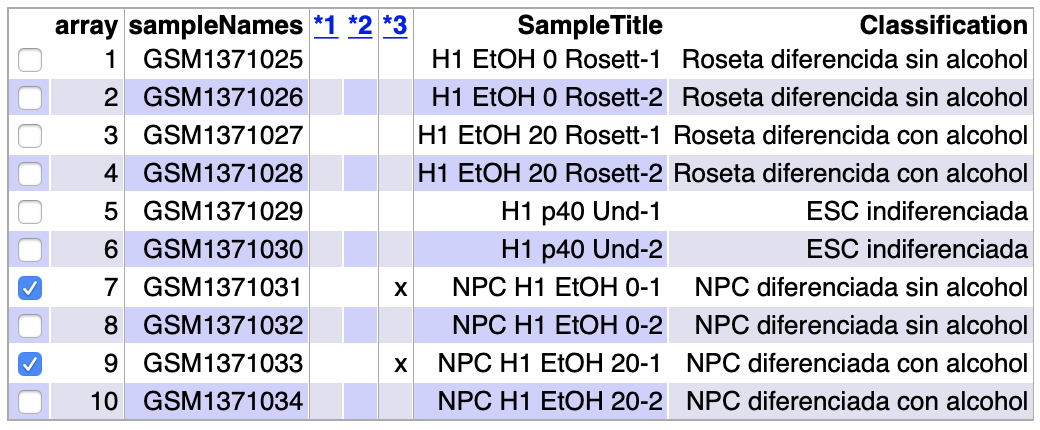
\includegraphics[width=14.44in]{figures/QCRawData} \caption{Tabla resumen del archivo index.html, generdo por el paquete arrayQualityMetrics en los datos crudos}\label{fig:QCRawDataRes}
\end{figure}

Los arrays 7 y 9 se consideran outliers a través de un plot MA, el cual
visualiza las diferencias entre las mediciones tomadas en dos muestras.
Sin embargo, ambos arrays los mantendré en el análisis puesto que solo
una de las tres pruebas no es suficiente para considerar suprimir dichos
arrays del análisis.

A continuación desarrollo el gráfico resultado del \textbf{Análisis de
Componentes Principales (PCA)}, donde se recogen los dos primeros
componentes principales.Dicho gráfico se recoge en el directorio
\emph{figures}.

\begin{Shaded}
\begin{Highlighting}[]
\KeywordTok{library}\NormalTok{(ggplot2)}
\KeywordTok{library}\NormalTok{(ggrepel)}
\NormalTok{plotPCA3 <-}\StringTok{ }\ControlFlowTok{function}\NormalTok{ (datos, labels, factor, title, scale,colores, }\DataTypeTok{size =} \FloatTok{1.5}\NormalTok{, }\DataTypeTok{glineas =} \FloatTok{0.25}\NormalTok{) \{}
\NormalTok{  data <-}\StringTok{ }\KeywordTok{prcomp}\NormalTok{(}\KeywordTok{t}\NormalTok{(datos),}\DataTypeTok{scale=}\NormalTok{scale)}
  \CommentTok{# plot adjustments}
\NormalTok{  dataDf <-}\StringTok{ }\KeywordTok{data.frame}\NormalTok{(data}\OperatorTok{$}\NormalTok{x)}
\NormalTok{  Group <-}\StringTok{ }\NormalTok{factor}
\NormalTok{  loads <-}\StringTok{ }\KeywordTok{round}\NormalTok{(data}\OperatorTok{$}\NormalTok{sdev}\OperatorTok{^}\DecValTok{2}\OperatorTok{/}\KeywordTok{sum}\NormalTok{(data}\OperatorTok{$}\NormalTok{sdev}\OperatorTok{^}\DecValTok{2}\NormalTok{)}\OperatorTok{*}\DecValTok{100}\NormalTok{,}\DecValTok{1}\NormalTok{)}
  \CommentTok{# main plot}
\NormalTok{  p1 <-}\StringTok{ }\KeywordTok{ggplot}\NormalTok{(dataDf,}\KeywordTok{aes}\NormalTok{(}\DataTypeTok{x=}\NormalTok{PC1, }\DataTypeTok{y=}\NormalTok{PC2)) }\OperatorTok{+}
\StringTok{    }\KeywordTok{theme_classic}\NormalTok{() }\OperatorTok{+}
\StringTok{    }\KeywordTok{geom_hline}\NormalTok{(}\DataTypeTok{yintercept =} \DecValTok{0}\NormalTok{, }\DataTypeTok{color =} \StringTok{"gray70"}\NormalTok{) }\OperatorTok{+}
\StringTok{    }\KeywordTok{geom_vline}\NormalTok{(}\DataTypeTok{xintercept =} \DecValTok{0}\NormalTok{, }\DataTypeTok{color =} \StringTok{"gray70"}\NormalTok{) }\OperatorTok{+}
\StringTok{    }\KeywordTok{geom_point}\NormalTok{(}\KeywordTok{aes}\NormalTok{(}\DataTypeTok{color =}\NormalTok{ Group), }\DataTypeTok{alpha =} \FloatTok{0.55}\NormalTok{, }\DataTypeTok{size =} \DecValTok{3}\NormalTok{) }\OperatorTok{+}
\StringTok{    }\KeywordTok{coord_cartesian}\NormalTok{(}\DataTypeTok{xlim =} \KeywordTok{c}\NormalTok{(}\KeywordTok{min}\NormalTok{(data}\OperatorTok{$}\NormalTok{x[,}\DecValTok{1}\NormalTok{])}\OperatorTok{-}\DecValTok{5}\NormalTok{,}\KeywordTok{max}\NormalTok{(data}\OperatorTok{$}\NormalTok{x[,}\DecValTok{1}\NormalTok{])}\OperatorTok{+}\DecValTok{5}\NormalTok{)) }\OperatorTok{+}
\StringTok{    }\KeywordTok{scale_fill_discrete}\NormalTok{(}\DataTypeTok{name =} \StringTok{"Group"}\NormalTok{)}
  \CommentTok{# avoiding labels superposition}
\NormalTok{  p1 }\OperatorTok{+}\StringTok{ }\KeywordTok{geom_text_repel}\NormalTok{(}\KeywordTok{aes}\NormalTok{(}\DataTypeTok{y =}\NormalTok{ PC2 }\OperatorTok{+}\StringTok{ }\FloatTok{0.25}\NormalTok{, }\DataTypeTok{label =}\NormalTok{ labels),}\DataTypeTok{segment.size =} \FloatTok{0.25}\NormalTok{, }\DataTypeTok{size =}\NormalTok{ size) }\OperatorTok{+}\StringTok{ }
\StringTok{    }\KeywordTok{labs}\NormalTok{(}\DataTypeTok{x =} \KeywordTok{c}\NormalTok{(}\KeywordTok{paste}\NormalTok{(}\StringTok{"PC1"}\NormalTok{,loads[}\DecValTok{1}\NormalTok{],}\StringTok{"%"}\NormalTok{)),}\DataTypeTok{y=}\KeywordTok{c}\NormalTok{(}\KeywordTok{paste}\NormalTok{(}\StringTok{"PC2"}\NormalTok{,loads[}\DecValTok{2}\NormalTok{],}\StringTok{"%"}\NormalTok{))) }\OperatorTok{+}\StringTok{  }
\StringTok{    }\KeywordTok{ggtitle}\NormalTok{(}\KeywordTok{paste}\NormalTok{(}\StringTok{"Análisis de componentes principales para: "}\NormalTok{,title,}\DataTypeTok{sep=}\StringTok{" "}\NormalTok{))}\OperatorTok{+}\StringTok{ }
\StringTok{    }\KeywordTok{theme}\NormalTok{(}\DataTypeTok{plot.title =} \KeywordTok{element_text}\NormalTok{(}\DataTypeTok{hjust =} \FloatTok{0.5}\NormalTok{)) }\OperatorTok{+}
\StringTok{    }\KeywordTok{scale_color_manual}\NormalTok{(}\DataTypeTok{values=}\NormalTok{colores)}
\NormalTok{  \}}
\end{Highlighting}
\end{Shaded}

\begin{Shaded}
\begin{Highlighting}[]
\KeywordTok{require}\NormalTok{(ggplot2)}
\KeywordTok{plotPCA3}\NormalTok{(}\KeywordTok{exprs}\NormalTok{(rawData), }\DataTypeTok{labels =}\NormalTok{ targets}\OperatorTok{$}\NormalTok{ShortName, }\DataTypeTok{factor =}\NormalTok{ targets}\OperatorTok{$}\NormalTok{Group, }
         \DataTypeTok{title=}\StringTok{"Datos crudos"}\NormalTok{, }\DataTypeTok{scale =} \OtherTok{FALSE}\NormalTok{, }\DataTypeTok{size =} \DecValTok{4}\NormalTok{, }
         \DataTypeTok{colores =} \KeywordTok{c}\NormalTok{(}\StringTok{"red"}\NormalTok{, }\StringTok{"blue"}\NormalTok{, }\StringTok{"green"}\NormalTok{, }\StringTok{"yellow"}\NormalTok{, }\StringTok{"pink"}\NormalTok{))}
\end{Highlighting}
\end{Shaded}

\begin{figure}
\centering
\includegraphics{Pipeline-del-análisis_files/figure-latex/PCARaw-1.pdf}
\caption{Visualization of the two first Principal Components for raw
data}
\end{figure}

El análisis de componentes principales indica que el 57,4\% de la
variabilidad total de las muestras se explica con el primer componente.
En el gráfico se observa cómo el factor \emph{tipo celular} es la
principal fuente de variabilidad, puesto que las células indiferenciadas
(p40) se encuentran a la derecha del gráfico mientras que las células
diferenciadas (NPC) se sitúan a la izquierda del mismo. Del mismo modo,
el tipo celular \emph{Rosetta} se encuentra en mitad del gráfico ya que
es el grupo intermedio entre las células madre embrionarias (p40) y las
células progenitoras neurales (NPC).

Existen otros gráficos que nos deja el control de calidad de los datos
en crudo, entre ellos destaca el boxplot múltiple con la distribución de
las intensidades a lo largo de todas las muestras.

\begin{figure}
\centering
\includegraphics{Pipeline-del-análisis_files/figure-latex/BoxplotRaw-1.pdf}
\caption{Boxplot para las intensidades de los arrays (Raw Data)}
\end{figure}

\begin{enumerate}
\def\labelenumi{\arabic{enumi}.}
\setcounter{enumi}{2}
\tightlist
\item
  Normalización de los datos crudos
\end{enumerate}

El objetivo de la normalización es hacer comparables los arrays entre sí
además de eliminar cualquier variabilidad en las muestras no debida a
razones biológicas. Es decir, la normalización de los datos asegura que
las diferencias de intensidades en las muestras se deban a diferencias
en la expresión de los genes y no a sesgos debidos a cuestiones técnicas
del experimento.

El proceso consta de tres etapas: eliminación del ruido de fondo,
normalización y sumarización de los datos. Los tres procesos se llevan a
cabo gracias al método \textbf{Robust Multichip Analysis} a través de la
función \emph{rma}.

\begin{Shaded}
\begin{Highlighting}[]
\NormalTok{eset_rma <-}\StringTok{ }\KeywordTok{rma}\NormalTok{(rawData)}
\end{Highlighting}
\end{Shaded}

\begin{verbatim}
## Background correcting
## Normalizing
## Calculating Expression
\end{verbatim}

Una vez tenemos los datos normalizados, repetimos el proceso de control
de calidad de los datos pero con los datos normalizados.

\begin{enumerate}
\def\labelenumi{\arabic{enumi}.}
\setcounter{enumi}{3}
\tightlist
\item
  Control de calidad de los datos normalizados
\end{enumerate}

El resultado del control de calidad de los datos normalizados los
podemos ver nuevamente en el archivo \textbf{index.html} de la carpeta
\emph{normalized\_quality} en el directorio \emph{results}. El resumen
del resultado se muestra en la siguiente tabla, donde se observan los
arrays 5 y 6 como outliers a través de la medida ``distancias entre
arrays''. Estos arrays se mantendrán en el análisis por la misma
justificación dada anteriormente, una sola prueba de las tres pruebas
realizadas para detectar outliers no es suficiente como para eliminar un
array del análisis.

\begin{figure}
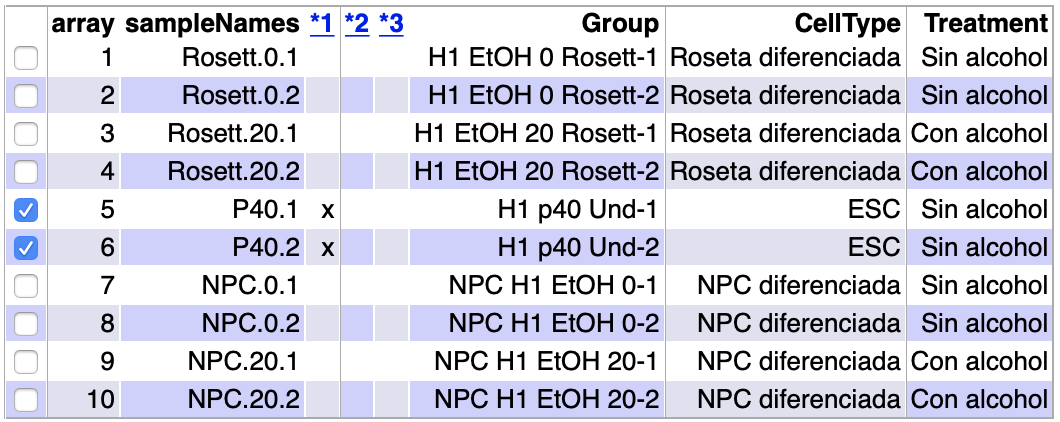
\includegraphics[width=14.72in]{figures/QCNormalizedData} \caption{Tabla resumen del archivo index.html, generdo por el paquete arrayQualityMetrics en los datos normalizados}\label{fig:QCNormDataRes}
\end{figure}

Se puede observar en el gráfico de \textbf{Componentes Principales} de
los datos normalizados que las muestras se siguen separando en función
al \emph{tipo celular}, indicando que este sigue siendo el factor
principal de variación entre las muestras y no el tratamiento con
alcohol. En este caso, dicho factor explica el 69,5\% de la variabilidad
total de las muestras.

\begin{Shaded}
\begin{Highlighting}[]
\KeywordTok{plotPCA3}\NormalTok{(}\KeywordTok{exprs}\NormalTok{(eset_rma), }\DataTypeTok{labels =}\NormalTok{ targets}\OperatorTok{$}\NormalTok{ShortName, }\DataTypeTok{factor =}\NormalTok{ targets}\OperatorTok{$}\NormalTok{Group, }
         \DataTypeTok{title=}\StringTok{"Datos normalizados"}\NormalTok{, }\DataTypeTok{scale =} \OtherTok{FALSE}\NormalTok{, }\DataTypeTok{size =} \DecValTok{4}\NormalTok{, }
         \DataTypeTok{colores =} \KeywordTok{c}\NormalTok{(}\StringTok{"red"}\NormalTok{, }\StringTok{"blue"}\NormalTok{, }\StringTok{"green"}\NormalTok{, }\StringTok{"yellow"}\NormalTok{, }\StringTok{"pink"}\NormalTok{))}
\end{Highlighting}
\end{Shaded}

\begin{figure}
\centering
\includegraphics{Pipeline-del-análisis_files/figure-latex/PCANorm-1.pdf}
\caption{Visualization of first two principal components for normalized
data}
\end{figure}

En el boxplot de intensidades de los datos normalizados se espera que
todos los boxplots tengan el mismo aspecto; es decir, las mismas
intensidades. Esto es debido a que en el proceso de normaliación se
incluye la normalización de los cuantiles, en el que la distribución
empírica de todas las muestras se establece con los mismos valores. Aquí
se muestra el boxplot de \textbf{Distribución de los valores de
intensidad de los datos normalizados}.

\begin{Shaded}
\begin{Highlighting}[]
\KeywordTok{boxplot}\NormalTok{(eset_rma, }\DataTypeTok{cex.axis=}\FloatTok{0.5}\NormalTok{, }\DataTypeTok{las=}\DecValTok{2}\NormalTok{,  }\DataTypeTok{which=}\StringTok{"all"}\NormalTok{, }
         \DataTypeTok{col =} \KeywordTok{c}\NormalTok{(}\KeywordTok{rep}\NormalTok{(}\StringTok{"red"}\NormalTok{, }\DecValTok{2}\NormalTok{), }\KeywordTok{rep}\NormalTok{(}\StringTok{"blue"}\NormalTok{, }\DecValTok{2}\NormalTok{), }\KeywordTok{rep}\NormalTok{(}\StringTok{"green"}\NormalTok{, }\DecValTok{2}\NormalTok{), }\KeywordTok{rep}\NormalTok{(}\StringTok{"yellow"}\NormalTok{, }\DecValTok{2}\NormalTok{), }\KeywordTok{rep}\NormalTok{(}\StringTok{"pink"}\NormalTok{,}\DecValTok{2}\NormalTok{)),}
         \DataTypeTok{main=}\StringTok{"Distribución de los valores de intensidad }\CharTok{\textbackslash{}n}\StringTok{ de los datos normalizados"}\NormalTok{)}
\end{Highlighting}
\end{Shaded}

\begin{figure}
\centering
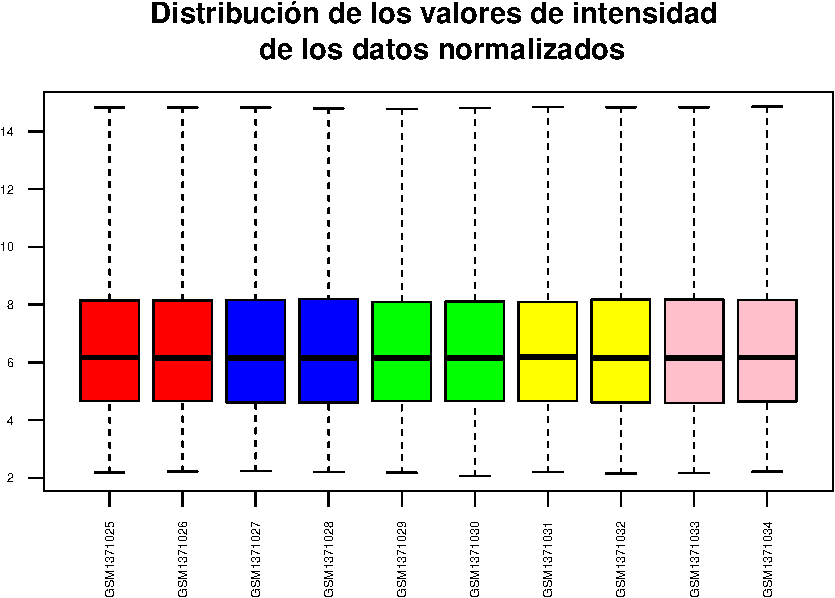
\includegraphics{Pipeline-del-análisis_files/figure-latex/BoxplotNormalized-1.pdf}
\caption{Boxplot para las intensidades de los arrays (Datos
Normalizados)}
\end{figure}

Un control que acompaña al análisis de componentes principales, es el
llamado \textbf{Batch Detection}. Este control consiste en conocer la
procedencia de la mayor fuente de variabilidad introducido por las
variaciones experimentales dependientes del tiempo y lugar del
experimento a la hora de recolectar y analizar las muestras.

Existen distintos métodos de llevar a cabo este control, uno de los más
conocidos es el llamado \textbf{Combat and Principal variation component
analysis (PVCA)}. Esta técnica estima la fuente y la proporción de la
variación en dos pasos, el análisis de componentes principales y el
análisis de componentes de variación.

En el gráfico de estimación de PVCA se muestra una barra por cada fuente
de variación incluída en el análisis. El gráfico indica que el factor
\emph{Group} es el de mayor variabilidad, al cual se le atribuye
aproximadamente el 79\% de la variación; esto coincide con lo observado
en los gráficos de componentes principales tanto de los datos en crudo
como de los datos normalizados. Además, se indica que el factor
\emph{Tratamiento con EtOH} tan sólo supone un 2,7\% de la variabilidad
de las muestras.

\begin{Shaded}
\begin{Highlighting}[]
\CommentTok{#plot the results}
\NormalTok{bp <-}\StringTok{ }\KeywordTok{barplot}\NormalTok{(pvcaObj}\OperatorTok{$}\NormalTok{dat, }\DataTypeTok{xlab =} \StringTok{"Factores"}\NormalTok{,}
  \DataTypeTok{ylab =} \StringTok{"Variación de la proporción media ponderada"}\NormalTok{,}
  \DataTypeTok{ylim=} \KeywordTok{c}\NormalTok{(}\DecValTok{0}\NormalTok{,}\FloatTok{1.1}\NormalTok{),}\DataTypeTok{col =} \KeywordTok{c}\NormalTok{(}\StringTok{"turquoise"}\NormalTok{), }\DataTypeTok{las=}\DecValTok{2}\NormalTok{,}
  \DataTypeTok{main=}\StringTok{"Estimación PVCA"}\NormalTok{)}
\KeywordTok{axis}\NormalTok{(}\DecValTok{1}\NormalTok{, }\DataTypeTok{at =}\NormalTok{ bp, }\DataTypeTok{labels =}\NormalTok{ pvcaObj}\OperatorTok{$}\NormalTok{label, }\DataTypeTok{cex.axis =} \FloatTok{0.55}\NormalTok{, }\DataTypeTok{las=}\DecValTok{2}\NormalTok{)}
\NormalTok{values =}\StringTok{ }\NormalTok{pvcaObj}\OperatorTok{$}\NormalTok{dat}
\NormalTok{new_values =}\StringTok{ }\KeywordTok{round}\NormalTok{(values , }\DecValTok{3}\NormalTok{)}
\KeywordTok{text}\NormalTok{(bp,pvcaObj}\OperatorTok{$}\NormalTok{dat,}\DataTypeTok{labels =}\NormalTok{ new_values, }\DataTypeTok{pos=}\DecValTok{3}\NormalTok{, }\DataTypeTok{cex =} \FloatTok{0.5}\NormalTok{)}
\end{Highlighting}
\end{Shaded}

\begin{figure}
\centering
\includegraphics{Pipeline-del-análisis_files/figure-latex/plotPVCA-1.pdf}
\caption{Relative importance of the different factors -genotype,
temperature and interaction- affecting gene expression}
\end{figure}

\begin{enumerate}
\def\labelenumi{\arabic{enumi}.}
\setcounter{enumi}{4}
\tightlist
\item
  Filtraje no específico
\end{enumerate}

El filtraje no específico es el proceso de identificación y filtración
de los genes que no se espera que se expresen diferencialmente, sino que
su variación pueda deberse a la variación aleatoria.

La función encargada de hacer esta tarea es \emph{nsFilter} del paquete
\textbf{genefilter}. El criterio para identificar los genes que no se
expresan diferencialmente de los que si lo hacen es un umbral dado por
la persona encargada de hacer el análisis. Además, la función
\emph{nsFilter} tiene una segunda función, la de eliminar las muestras
que no tienen un identificador de genes asociado.

Antes de realizar el filtraje debemos conocer el tipo de microarray
utilizado y, posteriormente, descargar la librería de anotaciones
asociada a dicho tipo de microarray. En este análisis, el microarray
utilizado corresponde con el modelo \emph{Affymetrix Human Genome U133
Plus 2.0 Array}.

\begin{Shaded}
\begin{Highlighting}[]
\CommentTok{#Descarga del paquete genefilter para la función nsfilter}
\KeywordTok{library}\NormalTok{(genefilter)}
\CommentTok{#Descarga de la libreria de anotaciones del microarray utilizado}
\KeywordTok{library}\NormalTok{(hgu133plus2.db)}
\KeywordTok{annotation}\NormalTok{(eset_rma) <-}\StringTok{ "hgu133plus2.db"}
\NormalTok{filtered <-}\StringTok{ }\KeywordTok{nsFilter}\NormalTok{(eset_rma, }
                     \DataTypeTok{require.entrez =} \OtherTok{TRUE}\NormalTok{, }\DataTypeTok{remove.dupEntrez =} \OtherTok{TRUE}\NormalTok{,}
                     \DataTypeTok{var.filter=}\OtherTok{TRUE}\NormalTok{, }\DataTypeTok{var.func=}\NormalTok{IQR, }\DataTypeTok{var.cutoff=}\FloatTok{0.75}\NormalTok{, }
                     \DataTypeTok{filterByQuantile=}\OtherTok{TRUE}\NormalTok{, }\DataTypeTok{feature.exclude =} \StringTok{"^AFFX"}\NormalTok{)}
\end{Highlighting}
\end{Shaded}

El filtraje nos devuelve los genes filtrados en un objeto llamado en
este caso \textbf{eset\_filtered}. La clase de este objeto sigue siendo
\emph{ExpressionSet}; ya que este objeto se ha obtenido a través de los
datos normalizados \emph{eset\_rma}, que a su vez se obtuvieron de los
datos en bruto \emph{rawData}, todos de la misma clase.

\begin{Shaded}
\begin{Highlighting}[]
\KeywordTok{print}\NormalTok{(filtered}\OperatorTok{$}\NormalTok{filter.log)}
\end{Highlighting}
\end{Shaded}

\begin{verbatim}
## $numDupsRemoved
## [1] 21738
## 
## $numLowVar
## [1] 15130
## 
## $numRemoved.ENTREZID
## [1] 12753
## 
## $feature.exclude
## [1] 10
\end{verbatim}

\begin{Shaded}
\begin{Highlighting}[]
\NormalTok{eset_filtered <-filtered}\OperatorTok{$}\NormalTok{eset}
\end{Highlighting}
\end{Shaded}

\begin{enumerate}
\def\labelenumi{\arabic{enumi}.}
\setcounter{enumi}{5}
\tightlist
\item
  Identificación de genes diferencialmente expresados
\end{enumerate}

Para identificar los genes diferencialmente expresados existen varios
métodos. Hasta el momento, el método aue mejores resultados ofrece es el
de \textbf{Modelos lineales para microarrays}. Dicho método está
implementado en el paquete \textbf{limma}.

El \textbf{primer paso} para el análisis basado en modelos lineales es
crear la \emph{matriz de diseño}, que es una tabla que describe la
asignación de cada muestra a un grupo o condición experimental. Tiene
tantas filas como muestras y tantas columnas como grupos, en este caso
hay cinco grupos si juntamos los dos factores: tipo celular y
tratamiento. Cada fila contiene un uno en la columna del grupo al que
pertenece la muestra y un cero en las demás.

La matriz de diseño se elabora a partir de los datos filtrados
\emph{eset\_filtered}. El resultado es el siguiente:

\begin{verbatim}
##    Rosett.0 Rosett.20 p40 NPC.0 NPC.20
## 1         1         0   0     0      0
## 2         1         0   0     0      0
## 3         0         1   0     0      0
## 4         0         1   0     0      0
## 5         0         0   1     0      0
## 6         0         0   1     0      0
## 7         0         0   0     1      0
## 8         0         0   0     1      0
## 9         0         0   0     0      1
## 10        0         0   0     0      1
## attr(,"assign")
## [1] 1 1 1 1 1
## attr(,"contrasts")
## attr(,"contrasts")$Group
## [1] "contr.treatment"
\end{verbatim}

Una vez hecha la matriz de diseño, el \textbf{segundo paso} es realizar
comparaciones entre los grupos de genes a través de la \emph{matriz de
contraste}. La matriz de contraste tendrá tantas columnas como
comparaciones se hagan y tantas filas como grupos existentes. Esta
matriz estará compuesta de 1 y -1 en las filas de grupos a comparar y
ceros en el resto.

Según el
\href{https://www.ncbi.nlm.nih.gov/pmc/articles/PMC5040434/}{artículo
del experimento},la correlación de la expresión génica con el
tratamiento con EtOH no fue lo suficientemente fuerte sobre el efecto de
la diferenciación. Por lo tanto, se decide analizar el conjunto de datos
para el efecto del EtOH en las células de la roseta y NPC por separado.

La matriz de contraste la he definido para realizar cuatro
comparaciones, dos comparaciones para cada tipo celular (Roseta y NPC),
con el fin de responder a las siguientes preguntas:

\textbf{Contrastes para las rosetas neurales:}

\begin{itemize}
\tightlist
\item
  Efecto de la diferenciación celular hacia rosetas neurales
\item
  Efecto del tratamineto con EtOH en rosetas neurales
\end{itemize}

\textbf{Contrastes para las células progenitoras neurales (NPC):}

\begin{itemize}
\tightlist
\item
  Efecto de la diferenciación celular hacia células progenitoras
  neurales
\item
  Efecto del tratamineto con EtOH en células progenitoras neurales
\end{itemize}

\begin{verbatim}
##            Contrasts
## Levels      p40vsRosett0 Rosett20vsRosett0 p40vsNPC0 NPC20vsNPC0
##   Rosett.0            -1                -1         0           0
##   Rosett.20            0                 1         0           0
##   p40                  1                 0         1           0
##   NPC.0                0                 0        -1          -1
##   NPC.20               0                 0         0           1
\end{verbatim}

Ahora que las matrices de diseño y contraste están creadas, puedo pasar
a estimar el modelo y hacer las pruebas de significación para decidir
qué genes se expresan diferencialmente en cada condición.

El método del paquete \emph{limma} para la selección de genes utiliza
modelos empíricos de Bayes para combinar una estimación de la
variabilidad basada en toda la matriz con estimaciones individuales
basadas en cada uno de los valores individuales. Los estadísticos de
prueba se utilizan para ordenar los genes de más a menos expresados.

Este método, además, controla el número de falsos positivos a través de
un ajsute de los p-valores por el método de \emph{Benjamini and
Hochberg}.

Finalmente, la información relevante para la posterior exploración de
los resultados se almacena en un objeto R de la clase \textbf{MArrayLM}
definido en el paquete \emph{limma}. El objeto se llamará
\textbf{fit.main}.

\begin{verbatim}
## [1] "MArrayLM"
## attr(,"package")
## [1] "limma"
\end{verbatim}

Para terminar con la identificación de los genes diferencialmente
expresados, debo obtener la lista de dichos genes. Esto se hace a través
de la función \textbf{topTable} del paquete \emph{limma}. La función
\emph{topTable} nos devolverá una lista de genes ordenados de menor a
mayor p-valor, lo que se traduce en genes de más a menos expresados
diferencialmente. Junto al estadístico p-valor aparecen otros
estadísticos, destacando el p-valor ajustado o el estadístico B, que es
el posterior logaritmo de probabilidades del gen de ser contra no ser
expresado diferencialmente.

Obtendré una tabla para cada uno de los cuatro contrastes llevados a
cabo.

\textbf{Comparación 1} (p40vsRosett0): Genes que cambian su expresión
entre células indiferenciadas y rosetas neurales.

\begin{Shaded}
\begin{Highlighting}[]
\NormalTok{topTab_p40vsRosett0 <-}\StringTok{ }\KeywordTok{topTable}\NormalTok{ (fit.main, }\DataTypeTok{number=}\KeywordTok{nrow}\NormalTok{(fit.main), }\DataTypeTok{coef=}\StringTok{"p40vsRosett0"}\NormalTok{, }\DataTypeTok{adjust=}\StringTok{"fdr"}\NormalTok{) }
\KeywordTok{head}\NormalTok{(topTab_p40vsRosett0)}
\end{Highlighting}
\end{Shaded}

\begin{verbatim}
##                 logFC   AveExpr         t      P.Value    adj.P.Val        B
## 206373_at   -7.247784 11.916089 -145.9622 5.563830e-15 2.806396e-11 23.80169
## 221086_s_at -7.053506  8.486889 -118.9733 2.849593e-14 4.155992e-11 22.79328
## 204069_at   -5.951557  9.496864 -115.2565 3.671996e-14 4.155992e-11 22.62029
## 206018_at   -8.175788 11.804071 -113.8389 4.053567e-14 4.155992e-11 22.55168
## 201012_at   -6.151703  9.144047 -113.6084 4.119738e-14 4.155992e-11 22.54038
## 212764_at   -6.997682 10.028004 -110.2744 5.226443e-14 4.393696e-11 22.37234
\end{verbatim}

\textbf{Comparación 2} (Rosett20vsRosett0): Genes que cambian su
expresión bajo el tratamiento con 20mM de EtOH en rosetas neurales.

\begin{Shaded}
\begin{Highlighting}[]
\NormalTok{topTab_Rosett20vsRosett0 <-}\StringTok{ }\KeywordTok{topTable}\NormalTok{ (fit.main, }\DataTypeTok{number=}\KeywordTok{nrow}\NormalTok{(fit.main), }\DataTypeTok{coef=}\StringTok{"Rosett20vsRosett0"}\NormalTok{, }\DataTypeTok{adjust=}\StringTok{"fdr"}\NormalTok{) }
\KeywordTok{head}\NormalTok{(topTab_Rosett20vsRosett0)}
\end{Highlighting}
\end{Shaded}

\begin{verbatim}
##                   logFC  AveExpr         t      P.Value   adj.P.Val        B
## 221019_s_at  -0.8904331 7.331574 -16.18214 2.157364e-07 0.001088174 7.255788
## 209875_s_at  -0.7385711 8.636895 -12.47501 1.606207e-06 0.004023319 5.686700
## 206552_s_at  -1.4997448 8.686413 -11.25229 3.519545e-06 0.004023319 5.014387
## 222549_at    -0.6611985 6.824317 -11.21858 3.600320e-06 0.004023319 4.994504
## 206924_at    -0.7477088 7.215421 -11.06771 3.988222e-06 0.004023319 4.904552
## 1555450_a_at -0.7991543 5.825407 -10.28585 6.919160e-06 0.005252623 4.412336
\end{verbatim}

\textbf{Comparación 3} (p40vsNPC0): Genes que cambian su expresión entre
células indiferenciadas y células progenitoras neurales.

\begin{Shaded}
\begin{Highlighting}[]
\NormalTok{topTab_p40vsNPC0 <-}\StringTok{ }\KeywordTok{topTable}\NormalTok{ (fit.main, }\DataTypeTok{number=}\KeywordTok{nrow}\NormalTok{(fit.main), }\DataTypeTok{coef=}\StringTok{"p40vsNPC0"}\NormalTok{, }\DataTypeTok{adjust=}\StringTok{"fdr"}\NormalTok{) }
\KeywordTok{head}\NormalTok{(topTab_p40vsNPC0)}
\end{Highlighting}
\end{Shaded}

\begin{verbatim}
##                 logFC   AveExpr         t      P.Value    adj.P.Val        B
## 206373_at   -7.793669 11.916089 -156.9557 3.114442e-15 1.570925e-11 24.14319
## 209988_s_at -8.534566  9.158885 -132.8936 1.177220e-14 1.988252e-11 23.38483
## 238878_at   -7.762829  9.563890 -127.9598 1.592695e-14 1.988252e-11 23.19516
## 207443_at   -7.559835  9.644671 -124.1422 2.028729e-14 1.988252e-11 23.03877
## 204069_at   -6.349737  9.496864 -122.9675 2.188834e-14 1.988252e-11 22.98885
## 221086_s_at -7.219977  8.486889 -121.7812 2.365089e-14 1.988252e-11 22.93755
\end{verbatim}

\textbf{Comparación 4} (NPC20vsNPC0): Genes que cambian su expresión
bajo el tratamiento con 20mM de EtOH en células progenitoras neurales.

\begin{Shaded}
\begin{Highlighting}[]
\NormalTok{topTab_NPC20vsNPC0 <-}\StringTok{ }\KeywordTok{topTable}\NormalTok{ (fit.main, }\DataTypeTok{number=}\KeywordTok{nrow}\NormalTok{(fit.main), }\DataTypeTok{coef=}\StringTok{"NPC20vsNPC0"}\NormalTok{, }\DataTypeTok{adjust=}\StringTok{"fdr"}\NormalTok{) }
\KeywordTok{head}\NormalTok{(topTab_NPC20vsNPC0)}
\end{Highlighting}
\end{Shaded}

\begin{verbatim}
##                   logFC   AveExpr         t      P.Value    adj.P.Val        B
## 206349_at    -1.3770890  8.688765 -20.54262 3.336970e-08 0.0001308226 9.509704
## 200650_s_at   0.9974532 12.828520  19.28520 5.479087e-08 0.0001308226 9.086425
## 213880_at    -1.1437077  7.626006 -18.44092 7.780882e-08 0.0001308226 8.779723
## 1556057_s_at -1.0640304  7.933443 -16.92764 1.519035e-07 0.0001547235 8.179092
## 201848_s_at   1.1429809  8.833883  16.72138 1.671371e-07 0.0001547235 8.091710
## 225342_at     1.1032601  9.176274  16.34496 1.995667e-07 0.0001547235 7.928574
\end{verbatim}

La primera columna de cada una de las tablas obtenidas contiene la
identificación del fabricante (Affymetrix) de cada conjunto de sondas;
mientras que el resto de columnas son variables numéricas y estadísticas
para indicar el cambio de pliegue del gen. Con estas tablas finalizaría
el proceso de identificación de los genes diferencialmente expresados.

\begin{enumerate}
\def\labelenumi{\arabic{enumi}.}
\setcounter{enumi}{5}
\tightlist
\item
  Anotación de los resultados
\end{enumerate}

El proceso de anotación consiste en relacionar los identificadores de la
primera columna de las tablas, los cuales corresponden a conjuntos de
sondas o tránscritos, con información más fácil de manejar como el
\emph{Gene Symbol}, \emph{Entrez Gene} o \emph{Gene description}. Es
decir, el proceso de anotación es la identificación de cada gen con cada
ID de Affymetrix, además de complementar dichos genes con la máxima
información posible encontrada en diferentes bases de datos.

Para realizar la anotación de los resultados, sigo una función de base
cuyas funciones serán:

-Identificar a la primera columna de las tablas obtenidas anteriormente
como \emph{PROBEID}, esta columna contiene las identificaciones de las
sondas de Affymetrix. -Asociar a cada sonda de Affymetrix los
identificadores \emph{SYMBOL}, \emph{ENTREZID} y \emph{GENENAME}
disponibles en el archivo de anotaciones del microarray utilizado.

El paquete de anotaciones para el microarray utilizado es
\textbf{hgu133plus2.db}. Una vez que creemos las nuevas tablas,
derivadas de las tablas obtenidas con \emph{topTab} y a las que se les
han añadido las anotaciones pertinentes, se guardarán en diferentes
archivos \emph{.csv} dentro del directorio \textbf{resultados}.

\begin{Shaded}
\begin{Highlighting}[]
\NormalTok{annotatedTopTable <-}\StringTok{ }\ControlFlowTok{function}\NormalTok{(topTab, anotPackage)}
\NormalTok{\{}
\NormalTok{  topTab <-}\StringTok{ }\KeywordTok{cbind}\NormalTok{(}\DataTypeTok{PROBEID=}\KeywordTok{rownames}\NormalTok{(topTab), topTab)}
\NormalTok{  myProbes <-}\StringTok{ }\KeywordTok{rownames}\NormalTok{(topTab)}
\NormalTok{  thePackage <-}\StringTok{ }\KeywordTok{eval}\NormalTok{(}\KeywordTok{parse}\NormalTok{(}\DataTypeTok{text =}\NormalTok{ anotPackage))}
\NormalTok{  geneAnots <-}\StringTok{ }\KeywordTok{select}\NormalTok{(thePackage, myProbes, }\KeywordTok{c}\NormalTok{(}\StringTok{"SYMBOL"}\NormalTok{, }\StringTok{"ENTREZID"}\NormalTok{, }\StringTok{"GENENAME"}\NormalTok{))}
\NormalTok{  annotatedTopTab<-}\StringTok{ }\KeywordTok{merge}\NormalTok{(}\DataTypeTok{x=}\NormalTok{geneAnots, }\DataTypeTok{y=}\NormalTok{topTab, }\DataTypeTok{by.x=}\StringTok{"PROBEID"}\NormalTok{, }\DataTypeTok{by.y=}\StringTok{"PROBEID"}\NormalTok{)}
\KeywordTok{return}\NormalTok{(annotatedTopTab)}
\NormalTok{\}}
\end{Highlighting}
\end{Shaded}

\begin{Shaded}
\begin{Highlighting}[]
\KeywordTok{require}\NormalTok{(hgu133plus2.db)}
\NormalTok{topAnnotated_p40vsRosett0 <-}\StringTok{ }\KeywordTok{annotatedTopTable}\NormalTok{(topTab_p40vsRosett0,}
\DataTypeTok{anotPackage=}\StringTok{"hgu133plus2.db"}\NormalTok{)}
\NormalTok{topAnnotated_Rosett20vsRosett0 <-}\StringTok{ }\KeywordTok{annotatedTopTable}\NormalTok{(topTab_Rosett20vsRosett0,}
\DataTypeTok{anotPackage=}\StringTok{"hgu133plus2.db"}\NormalTok{)}
\NormalTok{topAnnotated_p40vsNPC0 <-}\StringTok{ }\KeywordTok{annotatedTopTable}\NormalTok{(topTab_p40vsNPC0,}
\DataTypeTok{anotPackage=}\StringTok{"hgu133plus2.db"}\NormalTok{)}
\NormalTok{topAnnotated_NPC20vsNPC0 <-}\StringTok{ }\KeywordTok{annotatedTopTable}\NormalTok{(topTab_NPC20vsNPC0,}
\DataTypeTok{anotPackage=}\StringTok{"hgu133plus2.db"}\NormalTok{)}
\KeywordTok{write.csv}\NormalTok{(topAnnotated_p40vsRosett0, }\DataTypeTok{file=}\StringTok{"./results/topAnnotated_p40vsRosett0.csv"}\NormalTok{)}
\KeywordTok{write.csv}\NormalTok{(topAnnotated_Rosett20vsRosett0, }\DataTypeTok{file=}\StringTok{"./results/topAnnotated_Rosett20vsRosett0.csv"}\NormalTok{)}
\KeywordTok{write.csv}\NormalTok{(topAnnotated_p40vsNPC0, }\DataTypeTok{file=}\StringTok{"./results/topAnnotated_p40vsNPC0.csv"}\NormalTok{)}
\KeywordTok{write.csv}\NormalTok{(topAnnotated_NPC20vsNPC0, }\DataTypeTok{file=}\StringTok{"./results/topAnnotated_NPC20vsNPC0.csv"}\NormalTok{)}
\end{Highlighting}
\end{Shaded}

Los resultados de las tablas de selección se pueden visualizar a través
de un gráfico llamado \textbf{volcano plot}. En este gráfico se
representa en el eje de abscisas los cambios de expresión en escala
logarítmica; mientras que en el eje de ordenadas se representa el
estadístico B o probabilidad del gen de estar contra la probabilidad de
no estar expresado diferencialmente (en escala logarítmica). En este
caso se representan los cuatro primeros genes más diferencialmente
expresados de cada tabla.

Los resultados se recogen en el archivo \emph{Volvanos.pdf} del
directorio \textbf{figures}.

\begin{enumerate}
\def\labelenumi{\arabic{enumi}.}
\setcounter{enumi}{7}
\tightlist
\item
  Comparación entre distintas comparaciones
\end{enumerate}

En este análisis se han realizado cuatro contrastes, dos contrastes para
las rosetas neurales y dos para las células progenitoras neurales. El
objetivo es extraer los genes que cambian simultáneamente entre las
distintas comparaciones para cada tipo celular por separado.

Para anotar y contar los genes que cambian en una o más condiciones se
utiliza la función \textbf{decideTest} del paquete \emph{limma}. Esta
función nos devolverá una tabla llamada \textbf{res} cuya interpretación
es la siguiente:

\begin{itemize}
\tightlist
\item
  1: El gen esta sobreexpresado (Up)
\item
  0: No hay cambio significativo en la expresión del gen (NotSig)
\item
  -1: El gen ha bajado su expresión (Down)
\end{itemize}

A continuación se muestra un resumen de la tabla \emph{res} obtenida,
donde ya puede observarse que el efecto de la diferenciación celular
(contrastes 1 y 3) es mucho más fuerte que el efecto del tratamiento con
EtOH (contrastes 2 y 4).

\begin{verbatim}
##        p40vsRosett0 Rosett20vsRosett0 p40vsNPC0 NPC20vsNPC0
## Down           2049                 5      2512          10
## NotSig         2590              5038      1899        5012
## Up              405                 1       633          22
\end{verbatim}

La representación visual de la tabla \emph{res} es un \textbf{Diagrama
de Venn} a través de la función \emph{VenDiagram}.

Como en este análisis se ha estudiado cada tipo celular por separado,
haré un Diagrama de Venn para las rosetas neurales y otro para las
células progenitoras neurales. Con este diagrama se encontrarán los
genes que han cambiado su expresión (tanto Upregulated como
Downregulated) en cada comparación y cuántos genes han cambiado su
expresión simultáneamente debido a los dos efectos: diferenciación
celular y tratamiento con EtOH.

\textbf{Diagrama de Venn para las rosetas neurales}

\begin{Shaded}
\begin{Highlighting}[]
\KeywordTok{vennDiagram}\NormalTok{ (res.selected[,}\KeywordTok{c}\NormalTok{(}\DecValTok{1}\NormalTok{,}\DecValTok{2}\NormalTok{)], }\DataTypeTok{cex=}\FloatTok{0.9}\NormalTok{, }\DataTypeTok{circle.col =} \StringTok{"lightpink"}\NormalTok{)}
\KeywordTok{title}\NormalTok{(}\StringTok{"Genes que cambian su expresión en Rosetas }\CharTok{\textbackslash{}n}\StringTok{ Genes seleccionados con FDR < 0.1 y logFC > 1"}\NormalTok{)}
\end{Highlighting}
\end{Shaded}

\begin{figure}
\centering
\includegraphics{Pipeline-del-análisis_files/figure-latex/vennDiagramRosett-1.pdf}
\caption{Venn diagram showing the genes in common between the three
performed for neural rosette}
\end{figure}

Del diagrama de Venn para las \emph{rosetas neurales} se obtienen las
siguientes conclusiones:

\begin{itemize}
\tightlist
\item
  Existen \(2449+5 = 2454\) genes que cambian su expresión por el efecto
  de la diferenciación celular desde H1 hESC hasta rosetas neurales.
\item
  Tan sólo \(5+1 = 6\) genes cambian su expresión por el efecto del
  tratamiento con 20mM de EtOH durante la diferenciación hacia rosetas
  neurales.
\item
  Un total de \(5\) genes ven alterada su expresión debido a la
  interación de ambas condiciones: diferenciación celular y tratamiento
  con EtOH.

  \begin{itemize}
  \tightlist
  \item
    \(1178\) genes no cambian sus perfiles de expresión ni por el efecto
    de la diferenciación celular ni por efecto del tratamiento con EtOH.
  \end{itemize}
\end{itemize}

\textbf{Diagrama de Venn para células progenitoras neurales (NPC)}

\begin{Shaded}
\begin{Highlighting}[]
\KeywordTok{vennDiagram}\NormalTok{ (res.selected[,}\KeywordTok{c}\NormalTok{(}\DecValTok{3}\NormalTok{,}\DecValTok{4}\NormalTok{)], }\DataTypeTok{cex=}\FloatTok{0.9}\NormalTok{, }\DataTypeTok{circle.col =} \StringTok{"lightblue"}\NormalTok{)}
\KeywordTok{title}\NormalTok{(}\StringTok{"Genes que cambian su expresión en NPC }\CharTok{\textbackslash{}n}\StringTok{ Genes seleccionados con FDR < 0.1 y logFC > 1"}\NormalTok{)}
\end{Highlighting}
\end{Shaded}

\begin{figure}
\centering
\includegraphics{Pipeline-del-análisis_files/figure-latex/vennDiagramNPC-1.pdf}
\caption{Venn diagram showing the genes in common between the
comparisons 3 and 4 performed}
\end{figure}

El diagrama de Venn para las \emph{NPC} nos deja los siguientes datos:

\begin{itemize}
\tightlist
\item
  Existen \(3122+23 = 3145\) genes que cambian su expresión por el
  efecto de la diferenciación celular desde H1 hESC hasta NPC.
\item
  Tan sólo \(23+9 = 32\) genes cambian su expresión por el efecto del
  tratamiento con 20mM de EtOH durante la diferenciación hacia NPC.
\item
  Un total de \(23\) genes ven alterada su expresión debido a la
  interación de ambas condiciones: diferenciación celular y tratamiento
  con EtOH en NPC.

  \begin{itemize}
  \tightlist
  \item
    \(479\) genes no cambian sus perfiles de expresión ni por el efecto
    de la diferenciación celular ni por efecto del tratamiento con EtOH
    en NPC.
  \end{itemize}
\end{itemize}

Las \textbf{conclusiones} que se obtiene de ambos diagramas es que el
efecto de la diferenciación celular es mucho más pronunciado por sí solo
que el hecho de que dicha diferenciación celular se produzca bajo el
tratamiento con 20mM de EtOH. Una segunda conclusión es que las NPC se
ven más afectadas que las rosetas neurales bajo el tratamiento con EtOH,
puesto que 32 genes cambian su expresión en NPC mientras que tan sólo 6
genes lo hacen en las rosetas neurales por efecto exclusivo de dicho
tratamiento.

Otra manera de visualizar los perfiles de expresión de los genes
seleccionados a través de la tabla \emph{res} es creando un
\textbf{Heatmap}. Dichos gráficos nos permiten visualizar las
expresiones de cada gen, pero esta vez si vamos a distinguir entre genes
\emph{up} o \emph{down} regulados. Además, tanto los genes seleccionados
como las 10 muestras se agruparán con el fin de encontrar grupos con
patrones de expresión similares.

El \emph{Heatmap} final se recoge en el directorio \textbf{figures} como
\emph{Heatmap.tiff}.

\begin{verbatim}
## 
## Attaching package: 'gplots'
\end{verbatim}

\begin{verbatim}
## The following object is masked from 'package:IRanges':
## 
##     space
\end{verbatim}

\begin{verbatim}
## The following object is masked from 'package:S4Vectors':
## 
##     space
\end{verbatim}

\begin{verbatim}
## The following object is masked from 'package:stats':
## 
##     lowess
\end{verbatim}

\#Tabla de anotaciones sencillas

Es posible hacer una tabla de anotaciones con hiperenlaces a las bases
de datos para cada anotación de los genes seleccionados anteriormente.
Esta tabla es posible gracias al paquete \textbf{annaffy} y el resultado
se recoge en un archivo llamado \emph{anotaciones.html} dentro del
directorio \textbf{resultados}.

\begin{enumerate}
\def\labelenumi{\arabic{enumi}.}
\setcounter{enumi}{8}
\tightlist
\item
  Análisis de significación biológica (``Gene Enrichment Analysis'')
\end{enumerate}

Una vez he seleccionado los genes que cambian su expresión entre las
diferentes comparaciones, debo darle un sentido biológico a dicha
selección. Además de los conocimientos biológicos necesarios para
resolver esta cuestión, existe una aproximación estadística llamada
\textbf{Gene Set Enrichment Analysis} que ayuda a interpretar la
significación biológica de estos genes.

El modo de operación del \emph{Gene Set Enrichment Analysis} es
identificar las funciones, rutas moleculares y procesos biológicos que
aparecen con mayor frecuencia entre las listas de los genes
seleccionados.

Existen distintos paquetes para llevar a cabo este análisis de
significación biológica, uno de ellos es el paquete de Bioconductor
\textbf{ReactomePA}. El paquete se basa en un modelo hipergeométrico
para evaluar si el número de genes seleccionados asociados a las vías es
mayor de lo esperado.

Los pasos a seguir serán preparar la lista de genes que van a ser
analizados (estos serán los diferentes contrastes realizados) y
asegurarnos de que en todas las listas exista el identificador
\emph{Entrez}.

\#Preparación de la lista de genes a analizar

Las listas de genes corresponden a los cuatro contrastes realizados. En
cada una de las cuatro listas se seleccionarán los genes cuyo p-valor
ajustado sea menor a 0.15. De estos genes seleccionados, se convertirá
su identificador en un identificador \emph{Entrez}, seleccionado a
partir de las anotaciones \emph{hgu133plus2} correspondientes al
microarray utilizado.

\begin{Shaded}
\begin{Highlighting}[]
\NormalTok{listOfTables <-}\StringTok{ }\KeywordTok{list}\NormalTok{(}\DataTypeTok{p40vsRosett0 =}\NormalTok{ topTab_p40vsRosett0,}
                     \DataTypeTok{Rosett20vsRosett0 =}\NormalTok{ topTab_Rosett20vsRosett0,}
                     \DataTypeTok{p40vsNPC0 =}\NormalTok{ topTab_p40vsNPC0,}
                     \DataTypeTok{NPC20vsNPC0 =}\NormalTok{ topTab_NPC20vsNPC0)}
\NormalTok{listOfSelected <-}\StringTok{ }\KeywordTok{list}\NormalTok{()}
\ControlFlowTok{for}\NormalTok{ (i }\ControlFlowTok{in} \DecValTok{1}\OperatorTok{:}\KeywordTok{length}\NormalTok{(listOfTables))\{}
  \CommentTok{# select the toptable}
\NormalTok{  topTab <-}\StringTok{ }\NormalTok{listOfTables[[i]]}
  \CommentTok{# select the genes to be included in the analysis}
\NormalTok{  whichGenes<-topTab[}\StringTok{"adj.P.Val"}\NormalTok{]}\OperatorTok{<}\FloatTok{0.15}
\NormalTok{  selectedIDs <-}\StringTok{ }\KeywordTok{rownames}\NormalTok{(topTab)[whichGenes]}
  \CommentTok{# convert the ID to Entrez}
\NormalTok{  EntrezIDs<-}\StringTok{ }\KeywordTok{select}\NormalTok{(hgu133plus2.db, selectedIDs, }\KeywordTok{c}\NormalTok{(}\StringTok{"ENTREZID"}\NormalTok{))}
\NormalTok{  EntrezIDs <-}\StringTok{ }\NormalTok{EntrezIDs}\OperatorTok{$}\NormalTok{ENTREZID}
\NormalTok{  listOfSelected[[i]] <-}\StringTok{ }\NormalTok{EntrezIDs}
  \KeywordTok{names}\NormalTok{(listOfSelected)[i] <-}\StringTok{ }\KeywordTok{names}\NormalTok{(listOfTables)[i]}
\NormalTok{\}}
\end{Highlighting}
\end{Shaded}

\begin{verbatim}
## 'select()' returned 1:1 mapping between keys and columns
## 'select()' returned 1:1 mapping between keys and columns
## 'select()' returned 1:1 mapping between keys and columns
## 'select()' returned 1:1 mapping between keys and columns
\end{verbatim}

\begin{Shaded}
\begin{Highlighting}[]
\KeywordTok{sapply}\NormalTok{(listOfSelected, length)}
\end{Highlighting}
\end{Shaded}

\begin{verbatim}
##      p40vsRosett0 Rosett20vsRosett0         p40vsNPC0       NPC20vsNPC0 
##              4747               542              4874              1403
\end{verbatim}

\#Preparación de los genes con anotaciones para el \emph{Homo sapiens}

En este estudio el organismo utilizado es el \emph{Homo sapiens}, por lo
que debemos indicar que los genes que han de mapearse tanto para las
anotaciones en GO como en KEEG corresponden a dicho organismo.

\begin{Shaded}
\begin{Highlighting}[]
\NormalTok{mapped_genes2GO <-}\StringTok{ }\KeywordTok{mappedkeys}\NormalTok{(org.Hs.egGO)}
\NormalTok{mapped_genes2KEGG <-}\StringTok{ }\KeywordTok{mappedkeys}\NormalTok{(org.Hs.egPATH)}
\NormalTok{mapped_genes <-}\StringTok{ }\KeywordTok{union}\NormalTok{(mapped_genes2GO , mapped_genes2KEGG)}
\end{Highlighting}
\end{Shaded}

\#Generación de los resultados

Gracias a la función \textbf{enrichPathway} del paquete
\emph{ReactomePA} se consigue obtener el análisis de significación
biológica. Esta función selecciona los genes cuyo p-valor es inferior a
0.05 dentro del universo de genes, que son todos los genes disponibles
en la anotación \textbf{org.Hs.eg} para el \emph{Homo sapines}.

\begin{Shaded}
\begin{Highlighting}[]
\KeywordTok{library}\NormalTok{(ReactomePA)}
\end{Highlighting}
\end{Shaded}

\begin{verbatim}
## 
\end{verbatim}

\begin{verbatim}
## Registered S3 method overwritten by 'enrichplot':
##   method               from
##   fortify.enrichResult DOSE
\end{verbatim}

\begin{verbatim}
## ReactomePA v1.30.0  For help: https://guangchuangyu.github.io/ReactomePA
## 
## If you use ReactomePA in published research, please cite:
## Guangchuang Yu, Qing-Yu He. ReactomePA: an R/Bioconductor package for reactome pathway analysis and visualization. Molecular BioSystems 2016, 12(2):477-479
\end{verbatim}

\begin{Shaded}
\begin{Highlighting}[]
\NormalTok{listOfData <-}\StringTok{ }\NormalTok{listOfSelected[}\DecValTok{1}\OperatorTok{:}\DecValTok{4}\NormalTok{]}
\NormalTok{comparisonsNames <-}\StringTok{ }\KeywordTok{names}\NormalTok{(listOfData)}
\NormalTok{universe <-}\StringTok{ }\NormalTok{mapped_genes}

\ControlFlowTok{for}\NormalTok{ (i }\ControlFlowTok{in} \DecValTok{1}\OperatorTok{:}\KeywordTok{length}\NormalTok{(listOfData))\{}
\NormalTok{  genesIn <-}\StringTok{ }\NormalTok{listOfData[[i]]}
\NormalTok{  comparison <-}\StringTok{ }\NormalTok{comparisonsNames[i]}
\NormalTok{  enrich.result <-}\StringTok{ }\KeywordTok{enrichPathway}\NormalTok{(}\DataTypeTok{gene =}\NormalTok{ genesIn,}
                                 \DataTypeTok{pvalueCutoff =} \FloatTok{0.05}\NormalTok{,}
                                 \DataTypeTok{readable =}\NormalTok{ T,}
                                 \DataTypeTok{pAdjustMethod =} \StringTok{"BH"}\NormalTok{,}
                                 \DataTypeTok{organism =} \StringTok{"human"}\NormalTok{,}
                                 \DataTypeTok{universe =}\NormalTok{ universe)}
  
  \KeywordTok{cat}\NormalTok{(}\StringTok{"##################################"}\NormalTok{)}
  \KeywordTok{cat}\NormalTok{(}\StringTok{"}\CharTok{\textbackslash{}n}\StringTok{Comparison: "}\NormalTok{, comparison,}\StringTok{"}\CharTok{\textbackslash{}n}\StringTok{"}\NormalTok{)}
  \KeywordTok{print}\NormalTok{(}\KeywordTok{head}\NormalTok{(enrich.result))}

  \ControlFlowTok{if}\NormalTok{ (}\KeywordTok{length}\NormalTok{(}\KeywordTok{rownames}\NormalTok{(enrich.result}\OperatorTok{@}\NormalTok{result)) }\OperatorTok{!=}\StringTok{ }\DecValTok{0}\NormalTok{) \{}
  \KeywordTok{write.csv}\NormalTok{(}\KeywordTok{as.data.frame}\NormalTok{(enrich.result), }
             \DataTypeTok{file =}\KeywordTok{paste0}\NormalTok{(}\StringTok{"./results/"}\NormalTok{,}\StringTok{"ReactomePA.Results."}\NormalTok{,comparison,}\StringTok{".csv"}\NormalTok{), }
             \DataTypeTok{row.names =} \OtherTok{FALSE}\NormalTok{)}
  
  \KeywordTok{pdf}\NormalTok{(}\DataTypeTok{file=}\KeywordTok{paste0}\NormalTok{(}\StringTok{"./results/"}\NormalTok{,}\StringTok{"ReactomePABarplot."}\NormalTok{,comparison,}\StringTok{".pdf"}\NormalTok{))}
    \KeywordTok{print}\NormalTok{(}\KeywordTok{barplot}\NormalTok{(enrich.result, }\DataTypeTok{showCategory =} \DecValTok{15}\NormalTok{, }\DataTypeTok{font.size =} \DecValTok{4}\NormalTok{, }
            \DataTypeTok{title =} \KeywordTok{paste0}\NormalTok{(}\StringTok{"Reactome Pathway Analysis for "}\NormalTok{, comparison,}\StringTok{". Barplot"}\NormalTok{)))}
  \KeywordTok{dev.off}\NormalTok{()}
  
  \KeywordTok{pdf}\NormalTok{(}\DataTypeTok{file =} \KeywordTok{paste0}\NormalTok{(}\StringTok{"./results/"}\NormalTok{,}\StringTok{"ReactomePAcnetplot."}\NormalTok{,comparison,}\StringTok{".pdf"}\NormalTok{))}
    \KeywordTok{print}\NormalTok{(}\KeywordTok{cnetplot}\NormalTok{(enrich.result, }\DataTypeTok{categorySize =} \StringTok{"geneNum"}\NormalTok{, }\DataTypeTok{schowCategory =} \DecValTok{15}\NormalTok{, }
         \DataTypeTok{vertex.label.cex =} \FloatTok{0.75}\NormalTok{))}
  \KeywordTok{dev.off}\NormalTok{()}
  
  \KeywordTok{pdf}\NormalTok{(}\DataTypeTok{file =} \KeywordTok{paste0}\NormalTok{(}\StringTok{"./results/"}\NormalTok{,}\StringTok{"ReactomePAemapplot."}\NormalTok{,comparison,}\StringTok{".pdf"}\NormalTok{))}
    \KeywordTok{print}\NormalTok{(}\KeywordTok{emapplot}\NormalTok{(enrich.result, }\DataTypeTok{categorySize =} \StringTok{"geneNum"}\NormalTok{, }\DataTypeTok{schowCategory =} \DecValTok{15}\NormalTok{, }
         \DataTypeTok{vertex.label.cex =} \FloatTok{0.75}\NormalTok{))}
  \KeywordTok{dev.off}\NormalTok{()}
\NormalTok{  \}}
\NormalTok{\}}
\end{Highlighting}
\end{Shaded}

\begin{verbatim}
## ##################################
## Comparison:  p40vsRosett0 
##                          ID                                 Description
## R-HSA-1474244 R-HSA-1474244           Extracellular matrix organization
## R-HSA-9006934 R-HSA-9006934      Signaling by Receptor Tyrosine Kinases
## R-HSA-3000171 R-HSA-3000171      Non-integrin membrane-ECM interactions
## R-HSA-216083   R-HSA-216083          Integrin cell surface interactions
## R-HSA-1474290 R-HSA-1474290                          Collagen formation
## R-HSA-1650814 R-HSA-1650814 Collagen biosynthesis and modifying enzymes
##               GeneRatio   BgRatio       pvalue     p.adjust       qvalue
## R-HSA-1474244  132/2496 301/10616 2.483537e-15 3.439698e-12 2.990701e-12
## R-HSA-9006934  177/2496 473/10616 2.768214e-12 1.916988e-09 1.666756e-09
## R-HSA-3000171   35/2496  59/10616 3.838557e-09 1.772134e-06 1.540810e-06
## R-HSA-216083    44/2496  85/10616 1.378495e-08 4.773040e-06 4.149997e-06
## R-HSA-1474290   45/2496  90/10616 3.746741e-08 1.037847e-05 9.023731e-06
## R-HSA-1650814   36/2496  67/10616 8.214807e-08 1.896251e-05 1.648726e-05
##                                                                                                                                                                                                                                                                                                                                                                                                                                                                                                                                                                                                                                                                                                                                                                                                                                                                                                                                                                                                                                                                                                                              geneID
## R-HSA-1474244                                                                                                                                                                                                                                                                 COL2A1/COL11A1/VCAM1/COL8A1/COL5A2/LUM/FBN2/COL4A6/HAPLN1/COL5A1/SCUBE3/FN1/CD47/TGFB2/CAPN6/COL4A2/TNC/COL12A1/ADAMTS9/FBN1/JAM2/NCAN/COL1A2/NCAM1/CAPN2/DMD/ITGAV/LTBP1/EFEMP1/SPP1/COL4A1/ITGB5/ADAMTS1/SPARC/F11R/LOX/MFAP5/ADAM12/FBLN1/BMP7/COLGALT2/CDH1/TIMP2/COL7A1/MMP2/ITGB8/COL13A1/PDGFA/NTN4/LRP4/SERPINE1/SDC1/COL4A5/NRXN1/LOXL1/ITGA2/ADAMTS18/LTBP2/THBS1/ADAM19/LOXL2/COL9A1/ADAMTS5/CAST/EFEMP2/CD44/LAMC1/CTSV/LOXL3/MMP24/ADAM9/MMP7/NID1/SDC2/BGN/DDR2/MATN3/COL1A1/A2M/JAM3/COL22A1/ITGB1/COL3A1/MMP16/CTSK/P3H1/ADAM17/CASK/COL9A2/LAMA1/LOXL4/EMILIN3/PRKCA/COL15A1/COL9A3/SDC3/COL26A1/PCOLCE/ICAM1/PSEN1/PHYKPL/COLGALT1/HSPG2/LAMB1/COL25A1/ITGAE/ICAM3/CRTAP/CASP3/TGFB1/FMOD/TLL2/ITGA5/PCOLCE2/ITGA8/ITGA4/COL18A1/P3H2/PDGFB/MMP9/MMP14/ADAMTS2/ADAMTS8/DST/LAMA5/COL16A1/SERPINH1/COL27A1/FBLN2/ITGA9/EMILIN2/P4HA2
## R-HSA-9006934 COL2A1/COL11A1/PDGFC/COL5A2/FLRT3/DUSP4/FGF8/FGFBP3/CXCL12/COL5A1/GABRB3/FN1/ESRP1/COL4A2/HBEGF/AKT3/KITLG/FGFR2/COL1A2/ITGAV/RPS6KA2/PCSK5/CAV1/SPP1/IRS4/COL4A1/SPHK1/MEF2C/CYFIP2/SPARC/APOE/FGF18/PRKCB/ERBB3/PAG1/SHC3/SPRED1/ADAM12/RPS6KA3/PIK3R3/ERBB4/FGF9/PAK2/PIK3R1/WASF3/SPRY2/THBS3/SPINT2/FYN/RALGDS/PDGFA/PAK3/SPRED2/COL4A5/FLT1/ITGA2/SH3GL2/WASF1/THBS1/COL9A1/SPRY1/ROCK2/LAMC1/DOCK7/CDC42/SPINT1/VEGFA/ADCYAP1R1/TIAM1/CYFIP1/DUSP6/PDE3B/GALNT3/COL1A1/WWOX/RALB/ABI2/ATP6V0E2/GRB2/GRB10/CUL5/VEGFC/ITGB1/GAB2/NRG1/MAPK13/COL3A1/EGF/PLAT/PRKCE/RAP1A/ADAM17/MAPK11/ITPR3/ADCYAP1/IRS1/NRP1/THEM4/KIDINS220/ATP6V0A2/NEDD4/ANOS1/COL9A2/TNS3/EGFR/AXL/ARHGEF7/LAMA1/GAB1/PTPN18/PRKCA/SOCS6/CSK/COL9A3/BTC/LYN/TRIB3/AKT1/VAV3/CYBA/PSEN1/SHC2/CDK5R1/GABRB2/KIT/PTPRO/RIT1/CREB1/STAM2/MAPK12/FRS2/PIK3C3/PTPRJ/LAMB1/PDGFRB/STAT6/NTRK2/PIK3CA/GABRG2/PDGFRA/LRIG1/BAIAP2/SHC1/DUSP3/MET/DNAL4/STMN1/GABRG3/DOCK3/APH1B/EPS15/PIK3CB/PTPRK/VRK3/THBS4/FGF19/PDGFB/MMP9/NRG3/SH2D2A/TCIRG1/JAK2/NTRK3/PPP2R1B/ITPR1/SH2B3/SHB/LAMA5/WASF2/SOS1/PRKACB/COL27A1/ITPR2/BDNF/DLG4/ATP6V1G2/DNM3
## R-HSA-3000171                                                                                                                                                                                                                                                                                                                                                                                                                                                                                                                                                                                                                                                                                                                                                                                                                                                                                                     COL2A1/COL11A1/COL5A2/COL4A6/COL5A1/FN1/COL4A2/TNC/COL1A2/DMD/ITGAV/COL4A1/ITGB5/PDGFA/NTN4/SDC1/COL4A5/NRXN1/ITGA2/THBS1/LAMC1/SDC2/DDR2/COL1A1/ITGB1/COL3A1/CASK/LAMA1/PRKCA/SDC3/HSPG2/LAMB1/TGFB1/PDGFB/LAMA5
## R-HSA-216083                                                                                                                                                                                                                                                                                                                                                                                                                                                                                                                                                                                                                                                                                                                                                                                                                                         COL2A1/VCAM1/COL8A1/COL5A2/LUM/COL4A6/COL5A1/FN1/CD47/COL4A2/TNC/FBN1/JAM2/COL1A2/ITGAV/SPP1/COL4A1/ITGB5/F11R/CDH1/COL7A1/ITGB8/COL13A1/COL4A5/ITGA2/THBS1/COL9A1/CD44/COL1A1/JAM3/ITGB1/COL3A1/COL9A2/COL9A3/ICAM1/HSPG2/ITGAE/ICAM3/ITGA5/ITGA8/ITGA4/COL18A1/COL16A1/ITGA9
## R-HSA-1474290                                                                                                                                                                                                                                                                                                                                                                                                                                                                                                                                                                                                                                                                                                                                                                                                  COL2A1/COL11A1/COL8A1/COL5A2/COL4A6/COL5A1/COL4A2/COL12A1/COL1A2/COL4A1/LOX/COLGALT2/COL7A1/COL13A1/COL4A5/LOXL1/LOXL2/COL9A1/CTSV/LOXL3/MMP7/COL1A1/COL22A1/COL3A1/P3H1/COL9A2/LOXL4/COL15A1/COL9A3/COL26A1/PCOLCE/COLGALT1/COL25A1/CRTAP/TLL2/PCOLCE2/COL18A1/P3H2/MMP9/ADAMTS2/DST/COL16A1/SERPINH1/COL27A1/P4HA2
## R-HSA-1650814                                                                                                                                                                                                                                                                                                                                                                                                                                                                                                                                                                                                                                                                                                                                                                                                                                                 COL2A1/COL11A1/COL8A1/COL5A2/COL4A6/COL5A1/COL4A2/COL12A1/COL1A2/COL4A1/COLGALT2/COL7A1/COL13A1/COL4A5/COL9A1/COL1A1/COL22A1/COL3A1/P3H1/COL9A2/COL15A1/COL9A3/COL26A1/PCOLCE/COLGALT1/COL25A1/CRTAP/TLL2/PCOLCE2/COL18A1/P3H2/ADAMTS2/COL16A1/SERPINH1/COL27A1/P4HA2
##               Count
## R-HSA-1474244   132
## R-HSA-9006934   177
## R-HSA-3000171    35
## R-HSA-216083     44
## R-HSA-1474290    45
## R-HSA-1650814    36
\end{verbatim}

\begin{verbatim}
## ##################################
## Comparison:  Rosett20vsRosett0 
##                          ID
## R-HSA-1474244 R-HSA-1474244
## R-HSA-3000178 R-HSA-3000178
## R-HSA-3000171 R-HSA-3000171
## R-HSA-216083   R-HSA-216083
## R-HSA-1474228 R-HSA-1474228
## R-HSA-2022090 R-HSA-2022090
##                                                                Description
## R-HSA-1474244                            Extracellular matrix organization
## R-HSA-3000178                                            ECM proteoglycans
## R-HSA-3000171                       Non-integrin membrane-ECM interactions
## R-HSA-216083                            Integrin cell surface interactions
## R-HSA-1474228                      Degradation of the extracellular matrix
## R-HSA-2022090 Assembly of collagen fibrils and other multimeric structures
##               GeneRatio   BgRatio       pvalue     p.adjust       qvalue
## R-HSA-1474244    41/290 301/10616 6.950093e-18 5.462773e-15 5.238175e-15
## R-HSA-3000178    18/290  76/10616 1.275950e-12 5.014484e-10 4.808318e-10
## R-HSA-3000171    15/290  59/10616 3.322878e-11 8.705941e-09 8.348003e-09
## R-HSA-216083     17/290  85/10616 9.866529e-11 1.938773e-08 1.859062e-08
## R-HSA-1474228    21/290 140/10616 1.801590e-10 2.832099e-08 2.715660e-08
## R-HSA-2022090    13/290  61/10616 7.316348e-09 9.584416e-07 9.190360e-07
##                                                                                                                                                                                                                                                                     geneID
## R-HSA-1474244 SPP1/LUM/LTBP2/COL8A1/COL12A1/COL4A1/COL5A1/TNC/MMP2/LOXL2/CD44/HAPLN1/TGFB2/ADAM12/FN1/A2M/ADAM19/LOX/LAMB1/DDR2/COL18A1/LAMC2/SERPINE1/ITGB5/ACTN1/ADAMTS1/ITGB1/COL9A2/LRP4/ITGAV/NRXN1/CTSK/ICAM3/CAPN6/COL1A1/SPARC/MFAP5/ADAMTS5/COL1A2/COL9A3/COL11A1
## R-HSA-3000178                                                                                                                                               LUM/COL4A1/COL5A1/TNC/HAPLN1/TGFB2/FN1/LAMB1/SERPINE1/ITGB5/ITGB1/COL9A2/LRP4/ITGAV/COL1A1/SPARC/COL1A2/COL9A3
## R-HSA-3000171                                                                                                                                                                   COL4A1/COL5A1/TNC/FN1/LAMB1/DDR2/LAMC2/ITGB5/ACTN1/ITGB1/ITGAV/NRXN1/COL1A1/COL1A2/COL11A1
## R-HSA-216083                                                                                                                                                        SPP1/LUM/COL8A1/COL4A1/COL5A1/TNC/CD44/FN1/COL18A1/ITGB5/ITGB1/COL9A2/ITGAV/ICAM3/COL1A1/COL1A2/COL9A3
## R-HSA-1474228                                                                                                                       SPP1/COL8A1/COL12A1/COL4A1/COL5A1/MMP2/CD44/FN1/A2M/LAMB1/COL18A1/LAMC2/ADAMTS1/COL9A2/CTSK/CAPN6/COL1A1/ADAMTS5/COL1A2/COL9A3/COL11A1
## R-HSA-2022090                                                                                                                                                                     COL8A1/COL12A1/COL4A1/COL5A1/LOXL2/LOX/COL18A1/LAMC2/COL9A2/COL1A1/COL1A2/COL9A3/COL11A1
##               Count
## R-HSA-1474244    41
## R-HSA-3000178    18
## R-HSA-3000171    15
## R-HSA-216083     17
## R-HSA-1474228    21
## R-HSA-2022090    13
\end{verbatim}

\begin{verbatim}
## ##################################
## Comparison:  p40vsNPC0 
##                          ID                            Description GeneRatio
## R-HSA-9006934 R-HSA-9006934 Signaling by Receptor Tyrosine Kinases  184/2548
## R-HSA-1474244 R-HSA-1474244      Extracellular matrix organization  126/2548
## R-HSA-112316   R-HSA-112316                        Neuronal System  158/2548
## R-HSA-3000171 R-HSA-3000171 Non-integrin membrane-ECM interactions   38/2548
## R-HSA-399956   R-HSA-399956              CRMPs in Sema3A signaling   15/2548
## R-HSA-2022928 R-HSA-2022928                    HS-GAG biosynthesis   22/2548
##                 BgRatio       pvalue     p.adjust       qvalue
## R-HSA-9006934 473/10616 1.199528e-13 1.657748e-10 1.416706e-10
## R-HSA-1474244 301/10616 3.155830e-12 2.180679e-09 1.863601e-09
## R-HSA-112316  413/10616 3.274638e-11 1.508517e-08 1.289173e-08
## R-HSA-3000171  59/10616 4.765929e-11 1.646628e-08 1.407203e-08
## R-HSA-399956   16/10616 6.080268e-09 1.680586e-06 1.436223e-06
## R-HSA-2022928  31/10616 4.268041e-08 9.830722e-06 8.401302e-06
##                                                                                                                                                                                                                                                                                                                                                                                                                                                                                                                                                                                                                                                                                                                                                                                                                                                                                                                                                                                                                                                                                                                                                                       geneID
## R-HSA-9006934 COL2A1/DUSP4/ESRP1/COL11A1/APOE/KITLG/FLRT3/PDGFC/COL5A2/FGFBP3/CXCL12/RPS6KA2/AKT3/ERBB3/PAG1/CDK5R1/CYFIP2/SPINT2/PDGFA/SPP1/PAK3/ERBB4/MEF2C/FGFR2/CDC42/RALGDS/FGF8/PIK3R1/SHC1/PAK2/PIK3R3/SPHK1/SHC3/ATP6V0E2/ARHGEF7/COL4A2/FGF9/GALNT3/FYN/ADCYAP1/KIDINS220/CYBA/NRP1/THBS3/ITGA2/LYN/KIT/FLT1/RPS6KA3/DUSP6/SPINT1/LAMA5/LAMC2/APH1B/MET/FN1/IRS4/PTPRO/GRB10/WASF1/ANOS1/WASF3/NRG1/PRKACB/ITPR3/SPRY1/HBEGF/MAPK13/SPRED2/COL4A5/SPARC/GABRB3/RAP1A/MAPK11/ADAM12/NTRK2/LAMB1/LRIG1/GAB2/SPRED1/DOCK7/GABRB2/AXL/VEGFA/SPRY2/FGF18/COL3A1/NTRK1/IRS1/ABI2/VEGFC/PDE3B/FGF19/ROCK2/BAIAP2/COL1A2/RALB/TRIB3/ITGAV/SH2B3/STAT6/PIK3CB/GAB1/SH3GL2/CSK/AKT1/CUL5/EGF/BDNF/WASF2/SHC2/CAV1/DNM3/PTPN18/ATP6V1G2/LAMC1/PIK3C3/PRKCE/STAM2/COL5A1/CREB1/PPP2R1B/WWOX/EPS15/THBS4/NRG3/CDK5/PDGFRA/THEM4/LAMA4/SOCS6/PRKCB/COL9A3/TCIRG1/NTRK3/JAK2/MAPK12/DLG4/RIT1/ADAM17/CYFIP1/PIK3CA/SOS1/GABRG2/THBS1/PSEN1/PCSK5/RPS6KA5/ATP6V0A2/DNAL4/STMN1/NTF3/SH2D2A/COL4A1/NEDD4/ADCYAP1R1/MMP9/COL27A1/COL9A2/FRS2/DUSP3/PLAT/SHB/DOCK3/EGFR/TGFA/GRB2/PTPRK/BTC/LAMA1/ITPR2/WWP1/ITGB1/GABRG3/COL1A1/TIAM1/TNS3/PDGFRB/COL9A1/VAV3/GABRA1/PRKCA/VRK3/PTPRJ
## R-HSA-1474244                                                                                                                                                                                                                                                                                                                                                   COL2A1/VCAM1/LUM/NCAN/COL11A1/COL4A6/CDH1/NCAM1/COL5A2/COL8A1/F11R/CD47/SCUBE3/JAM2/PDGFA/SPP1/TGFB2/ITGB8/COL13A1/ADAMTS9/CTSV/TIMP2/CAPN6/HAPLN1/CAPN2/COL4A2/COL12A1/P3H2/ITGA2/SDC4/LAMA5/LAMC2/DMD/NTN4/FN1/COL18A1/CASK/FBN1/FBN2/PCOLCE2/COL4A5/SPARC/PCOLCE/ADAM12/LOX/ADAMTS1/LOXL3/JAM3/SERPINH1/LAMB1/COLGALT2/SDC3/COL22A1/ACTN1/FBLN1/ICAM3/COL3A1/ADAMTS5/LRP4/COL1A2/CRTAP/ITGAV/BGN/P4HA2/DDR2/ITGAE/LOXL1/MMP16/LAMC1/ADAM9/COL5A1/EMILIN2/MMP24/ADAMTS18/ADAMTS8/COL16A1/HSPG2/LAMA4/TNC/PHYKPL/COL9A3/A2M/EMILIN3/ITGA8/ADAM17/COL7A1/THBS1/PSEN1/LOXL4/LOXL2/BSG/SDC1/EFEMP2/MATN3/COL15A1/COL4A1/MFAP5/COL26A1/ITGA9/NRXN1/CTSK/MMP9/COL27A1/COL9A2/CASP3/DST/FBLN2/CAST/LAMA1/TGFB1/ITGB1/P3H1/COL1A1/COL25A1/NID2/NID1/CD44/COLGALT1/COL9A1/EFEMP1/LTBP2/ADAMTS2/TNR/SDC2/ITGB5/PRKCA
## R-HSA-112316                                                                                                                GRIA2/NCALD/GNG2/GNG3/RPS6KA2/GNG11/SNAP25/APBA2/SLC1A2/NLGN1/NEFL/GLRB/GNG4/NRXN3/SLITRK1/ERBB4/KCNC1/GRIA1/ABAT/ALDH5A1/PPM1E/MAPT/SLC32A1/SLC1A3/ARHGEF7/TSPAN7/PRKAA2/NRXN2/SYT1/SLITRK6/EPB41L5/RPS6KA3/PPFIA2/STXBP1/NRG1/CASK/PRKACB/CAMK4/TUBB3/HCN3/CACNA1B/KCNQ2/SLITRK5/KCNH8/GABRB3/TUBA1A/CHRNA3/GRIP1/GAD1/EPB41L1/ARHGEF9/PTPRD/KCNQ3/EPB41L2/SHANK2/GNG8/TUBB2A/LRRTM2/GABRB2/HOMER2/CACNB3/RIMS1/CAMK2D/GAD2/KCNB1/SLC6A1/ADCY6/BEGAIN/BCHE/GNB1/PANX1/HOMER3/KCND3/PRKAR1A/DLGAP4/CACNB2/COMT/ARL6IP5/PPFIA4/TSPOAP1/GRIA3/GABBR2/SLITRK4/LRRC7/DLG2/KCNB2/KCNK10/SYT9/KCNN3/GNAL/SLC1A6/CREB1/CACNG4/TUBB4B/GJC1/KCNK6/PRKCB/GNB5/NTRK3/CAMK2B/GRIK2/TUBB2B/EPB41L3/GABBR1/DLG4/LRFN3/GRM1/KCNK2/KCNQ4/GABRG2/IL1RAPL1/SHANK3/KCNMA1/PRKX/GRIK1/SYT12/KCNA2/STX1A/GNG12/KCNJ10/PPFIBP2/KCNJ4/GNAI1/NRXN1/PRKAA1/GLS/ABCC8/MAOA/SIPA1L1/KCNK3/KCNJ8/SLC1A1/KCNQ5/KCNJ9/ADCY2/TUBB6/LRRTM4/GABRG3/CHRNA9/PLCB1/APBA1/LIN7B/KCNMB4/KCNG1/CACNG2/KCNH2/TUBB4A/RAB3A/KCNA5/HCN4/CACNA2D3/CPLX1/SYN1/VAMP2/GABRA1/KCNJ2/LIN7A/PRKCA
## R-HSA-3000171                                                                                                                                                                                                                                                                                                                                                                                                                                                                                                                                                                                                                                                                                                                                                                                                                                                                                                                             COL2A1/COL11A1/COL4A6/COL5A2/PDGFA/COL4A2/ITGA2/SDC4/LAMA5/LAMC2/DMD/NTN4/FN1/CASK/COL4A5/LAMB1/SDC3/ACTN1/COL3A1/COL1A2/ITGAV/DDR2/LAMC1/COL5A1/HSPG2/LAMA4/TNC/THBS1/SDC1/COL4A1/NRXN1/LAMA1/TGFB1/ITGB1/COL1A1/SDC2/ITGB5/PRKCA
## R-HSA-399956                                                                                                                                                                                                                                                                                                                                                                                                                                                                                                                                                                                                                                                                                                                                                                                                                                                                                                                                                                                                                                                                 DPYSL4/CDK5R1/CRMP1/FYN/NRP1/PLXNA1/DPYSL5/DPYSL3/GSK3B/PLXNA2/DPYSL2/PLXNA3/SEMA3A/CDK5/PLXNA4
## R-HSA-2022928                                                                                                                                                                                                                                                                                                                                                                                                                                                                                                                                                                                                                                                                                                                                                                                                                                                                                                                                                                                                                            EXT1/HS6ST2/HS3ST1/GPC1/GPC6/SDC4/HS2ST1/HS3ST3A1/GPC2/SDC3/NDST4/HS6ST3/GPC3/HSPG2/SLC35D2/SDC1/GLCE/GPC4/NDST3/HS3ST2/HS3ST4/SDC2
##               Count
## R-HSA-9006934   184
## R-HSA-1474244   126
## R-HSA-112316    158
## R-HSA-3000171    38
## R-HSA-399956     15
## R-HSA-2022928    22
\end{verbatim}

\begin{verbatim}
## ##################################
## Comparison:  NPC20vsNPC0 
##                          ID                              Description GeneRatio
## R-HSA-3000171 R-HSA-3000171   Non-integrin membrane-ECM interactions    23/743
## R-HSA-1474244 R-HSA-1474244        Extracellular matrix organization    57/743
## R-HSA-9006934 R-HSA-9006934   Signaling by Receptor Tyrosine Kinases    71/743
## R-HSA-3000178 R-HSA-3000178                        ECM proteoglycans    20/743
## R-HSA-1474228 R-HSA-1474228  Degradation of the extracellular matrix    28/743
## R-HSA-6794362 R-HSA-6794362 Protein-protein interactions at synapses    21/743
##                 BgRatio       pvalue     p.adjust       qvalue
## R-HSA-3000171  59/10616 2.530799e-12 1.509679e-09 1.375924e-09
## R-HSA-1474244 301/10616 2.700677e-12 1.509679e-09 1.375924e-09
## R-HSA-9006934 473/10616 4.644724e-10 1.730934e-07 1.577576e-07
## R-HSA-3000178  76/10616 1.598340e-07 4.467359e-05 4.071560e-05
## R-HSA-1474228 140/10616 3.343902e-07 7.196692e-05 6.559079e-05
## R-HSA-6794362  87/10616 3.862268e-07 7.196692e-05 6.559079e-05
##                                                                                                                                                                                                                                                                                                                                                                                                                                                      geneID
## R-HSA-3000171                                                                                                                                                                                                                                                                                                    COL4A6/LAMC1/COL5A2/COL4A2/NRXN1/DMD/FN1/ITGB5/COL2A1/PRKCA/TGFB1/TNC/LAMC2/COL1A2/COL11A1/PDGFA/DDR2/COL4A5/SDC1/COL4A1/SDC2/ITGB1/COL5A1
## R-HSA-1474244                                                                                    LUM/COL4A6/FBN2/CAPN6/LAMC1/SPP1/HAPLN1/EFEMP2/NID2/MFAP5/P4HA2/VCAM1/PCOLCE2/CDH1/COL5A2/NCAN/COL4A2/NRXN1/FBN1/DMD/FN1/ITGB5/ADAM12/ADAMTS9/COL2A1/ADAMTS18/COL26A1/TLL2/SERPINH1/TGFB2/PRKCA/TGFB1/TNC/LAMC2/COL8A1/CASP3/COL1A2/COL7A1/SCUBE3/CRTAP/BGN/TNR/COL11A1/PDGFA/CTSK/DDR2/NID1/ITGB8/LOXL2/COL4A5/SDC1/COL4A1/SDC2/ITGB1/A2M/COLGALT2/COL5A1
## R-HSA-9006934 FGFR2/ANOS1/DUSP6/SPRY2/SPRY1/VEGFA/FGF8/LYN/LAMC1/KITLG/PRKCB/SPP1/IRS4/SPRED2/VEGFC/NTRK2/ERBB4/COL5A2/COL4A2/TIAM1/AXL/PAG1/FN1/ADAM12/CAV1/ESRP1/COL2A1/ADCYAP1R1/SHC2/BAIAP2/MET/PRKCA/CYFIP2/SHB/STMN1/LAMC2/PCSK5/IRS1/SPHK1/ARHGEF7/CDC42/COL1A2/FLRT3/CXCL12/CDK5R1/KIT/TNS3/ATP6V0E2/TGFA/SHC3/COL11A1/GABRB2/PDGFA/GALNT3/PTPN18/ERBB3/BTC/COL4A5/DNM3/LRIG1/PDGFRA/COL4A1/ADCYAP1/VAV3/NTRK1/ITGB1/BDNF/RPS6KA5/TRIB3/COL5A1/CYBA
## R-HSA-3000178                                                                                                                                                                                                                                                                                                                         LUM/COL4A6/LAMC1/HAPLN1/COL5A2/NCAN/COL4A2/FN1/ITGB5/COL2A1/TGFB2/TGFB1/TNC/COL1A2/BGN/TNR/COL4A5/COL4A1/ITGB1/COL5A1
## R-HSA-1474228                                                                                                                                                                                                                                                              COL4A6/FBN2/CAPN6/LAMC1/SPP1/CDH1/COL5A2/COL4A2/FBN1/FN1/ADAMTS9/COL2A1/ADAMTS18/COL26A1/TLL2/LAMC2/COL8A1/CASP3/COL1A2/COL7A1/SCUBE3/COL11A1/CTSK/NID1/COL4A5/COL4A1/A2M/COL5A1
## R-HSA-6794362                                                                                                                                                                                                                                                                                              PPFIA4/EPB41L1/SLITRK1/LRRTM4/NRXN1/NRXN3/SHANK2/SYT12/NRXN2/STXBP1/PTPRD/PPFIA2/HOMER2/PPFIBP2/BEGAIN/GRIA3/GRIA1/LIN7B/SIPA1L1/SLITRK6/SLITRK4
##               Count
## R-HSA-3000171    23
## R-HSA-1474244    57
## R-HSA-9006934    71
## R-HSA-3000178    20
## R-HSA-1474228    28
## R-HSA-6794362    21
\end{verbatim}

Una vez el análisis de significación ha finalizado, obtenemos cuatro
tipos de documentos para cada una de las cuatro comparaciones:

\begin{itemize}
\tightlist
\item
  Un \textbf{archivo excel} de extensión \emph{.csv} donde se resumen de
  todas las vías enriquecidas en cada proceso y sus correspondientes
  estadísticos.
\item
  Un \textbf{barplot} que recoge las mejores vías enriquecidas en cada
  proceso. La altura de cada barra corresponde al número de genes que
  están relacionados con dicha ruta metabólica enriquecida. Además, las
  vías están ordenadas en función de su significación estadística.
\item
  Un \textbf{cnetplot} que representa la red de vías enriquecidas en
  cada proceso, donde se incluyen las relaciones entre los genes
  incluídos en dichas vías. Este plot permite extraer la compleja
  relación entre los distintos genes y las enfermedades asociadas.
\item
  Un \textbf{emapplot} donde nuevamente se visualizan los genes en forma
  de red, en este caso los conjuntos de genes que se superponen
  mutuamente tienden a agruparse para facilitar su interpretación.
\end{itemize}

Para este estudio se han analizado cuatro comparaciones o conjuntos de
genes, los cuales, además, incluyen una enorme cantidad de genes. Para
tener una visión más clara de los resultados del análisis de
significación biológica, he construído una tabla para cada comparación
donde se resumen las cinco vías más enriquecidas y sus estadísticos. Sin
embargo, ya podemos adelantar que en las cuatro situaciones analizadas
la ruta de organización de la matriz extracelular se encuentra muy
enriquecida.

\emph{Tabla resumen para p40vsRosett0}

\begin{longtable}[]{@{}llllll@{}}
\caption{First rows and columns for Reactome results on p40vsRosett0.csv
comparison}\tabularnewline
\toprule
& Description & GeneRatio & BgRatio & pvalue & p.adjust\tabularnewline
\midrule
\endfirsthead
\toprule
& Description & GeneRatio & BgRatio & pvalue & p.adjust\tabularnewline
\midrule
\endhead
R-HSA-1474244 & Extracellular matrix organization & 132/2496 & 301/10616
& 2.48353664965071e-15 & 3.43969825976623e-12\tabularnewline
R-HSA-9006934 & Signaling by Receptor Tyrosine Kinases & 177/2496 &
473/10616 & 2.76821416020616e-12 & 1.91698830594277e-09\tabularnewline
R-HSA-3000171 & Non-integrin membrane-ECM interactions & 35/2496 &
59/10616 & 3.83855674324901e-09 & 1.77213369646662e-06\tabularnewline
R-HSA-216083 & Integrin cell surface interactions & 44/2496 & 85/10616 &
1.37849541626087e-08 & 4.77304037880326e-06\tabularnewline
R-HSA-1474290 & Collagen formation & 45/2496 & 90/10616 &
3.74674126835196e-08 & 1.03784733133349e-05\tabularnewline
\bottomrule
\end{longtable}

\emph{Tabla resumen para Rosett20vsRosett0}

\begin{longtable}[]{@{}llllll@{}}
\caption{First rows and columns for Reactome results on
Rosett20vsRosett0.csv comparison}\tabularnewline
\toprule
& Description & GeneRatio & BgRatio & pvalue & p.adjust\tabularnewline
\midrule
\endfirsthead
\toprule
& Description & GeneRatio & BgRatio & pvalue & p.adjust\tabularnewline
\midrule
\endhead
R-HSA-1474244 & Extracellular matrix organization & 41/290 & 301/10616 &
6.95009314084962e-18 & 5.4627732087078e-15\tabularnewline
R-HSA-3000178 & ECM proteoglycans & 18/290 & 76/10616 &
1.27595018881832e-12 & 5.01448424205601e-10\tabularnewline
R-HSA-3000171 & Non-integrin membrane-ECM interactions & 15/290 &
59/10616 & 3.32287817292416e-11 & 8.7059408130613e-09\tabularnewline
R-HSA-216083 & Integrin cell surface interactions & 17/290 & 85/10616 &
9.86652937566947e-11 & 1.93877302231905e-08\tabularnewline
R-HSA-1474228 & Degradation of the extracellular matrix & 21/290 &
140/10616 & 1.80158983714342e-10 & 2.83209922398945e-08\tabularnewline
\bottomrule
\end{longtable}

\emph{Tabla resumen para p40vsNPC0}

\begin{longtable}[]{@{}llllll@{}}
\caption{First rows and columns for Reactome results on p40vsNPC0.csv
comparison}\tabularnewline
\toprule
& Description & GeneRatio & BgRatio & pvalue & p.adjust\tabularnewline
\midrule
\endfirsthead
\toprule
& Description & GeneRatio & BgRatio & pvalue & p.adjust\tabularnewline
\midrule
\endhead
R-HSA-9006934 & Signaling by Receptor Tyrosine Kinases & 184/2548 &
473/10616 & 1.199527923865e-13 & 1.65774759078143e-10\tabularnewline
R-HSA-1474244 & Extracellular matrix organization & 126/2548 & 301/10616
& 3.15583025702968e-12 & 2.18067870760751e-09\tabularnewline
R-HSA-112316 & Neuronal System & 158/2548 & 413/10616 &
3.27463790914985e-11 & 1.50851653014836e-08\tabularnewline
R-HSA-3000171 & Non-integrin membrane-ECM interactions & 38/2548 &
59/10616 & 4.7659285783892e-11 & 1.64662832383347e-08\tabularnewline
R-HSA-399956 & CRMPs in Sema3A signaling & 15/2548 & 16/10616 &
6.08026782429621e-09 & 1.68058602663547e-06\tabularnewline
\bottomrule
\end{longtable}

\emph{Tabla resumen para NPC20vsNPC0}

\begin{longtable}[]{@{}llllll@{}}
\caption{First rows and columns for Reactome results on NPC20vsNPC0.csv
comparison}\tabularnewline
\toprule
& Description & GeneRatio & BgRatio & pvalue & p.adjust\tabularnewline
\midrule
\endfirsthead
\toprule
& Description & GeneRatio & BgRatio & pvalue & p.adjust\tabularnewline
\midrule
\endhead
R-HSA-3000171 & Non-integrin membrane-ECM interactions & 23/743 &
59/10616 & 2.53079932659888e-12 & 1.50967852505011e-09\tabularnewline
R-HSA-1474244 & Extracellular matrix organization & 57/743 & 301/10616 &
2.70067714678017e-12 & 1.50967852505011e-09\tabularnewline
R-HSA-9006934 & Signaling by Receptor Tyrosine Kinases & 71/743 &
473/10616 & 4.64472384774152e-10 & 1.73093375392501e-07\tabularnewline
R-HSA-3000178 & ECM proteoglycans & 20/743 & 76/10616 &
1.59833958740309e-07 & 4.46735914679163e-05\tabularnewline
R-HSA-1474228 & Degradation of the extracellular matrix & 28/743 &
140/10616 & 3.3439024171866e-07 & 7.19669238424329e-05\tabularnewline
\bottomrule
\end{longtable}

\end{document}
